\chapter{\scshape Implementazione del Sistema}\label{cap:3-implementazione}

\section{Struttura del progetto e Stack Tecnologico}
Un'architettura modulare produce i suoi benefici solo se la stessa separazione delle responsabilità si ritrova nell'organizzazione \textbf{fisica} del codice sorgente.
Per questo motivo l'implementazione è partita dalla definizione di una struttura di cartelle coerente con i moduli logici del sistema introdotti nel Capitolo~\ref{cap:2.2-architettura}, permettendo anche di facilitare la manutenzione e l'estendibilità futura del progetto.
Il progetto è organizzato come un \textbf{unico repository (\textit{monorepo})} che contiene, in tre cartelle di primo livello, il servizio di backend, l'applicazione web di frontend e i sorgenti \LaTeX{} del presente elaborato.
Questa scelta consente di \textbf{versionare} attraverso l'uso di strumenti di controllo della versione come \textit{Git} in modo coordinato le modifiche che attraversano più livelli, come l'aggiunta di un campo a un \textit{contratto di risposta} che deve essere recepito contemporaneamente dal server e dal client.
La struttura dei due componenti software è riportata in Figura~\ref{fig:strutturaRepository}.

\begin{figure}[htbp]
    \centering
    \begin{minipage}[t]{0.48\textwidth}
    \dirtree{%
    .1 backend/.
    .2 main.py.
    .2 requirements.txt.
    .2 \textit{.env}.
    .2 .env.example.
    .2 core/.
    .3 id\_card.py.
    .3 face\_detector.py.
    .3 face\_recognizer.py.
    .3 liveness.py.
    .2 api/.
    .3 routes.py.
    .3 register.py.
    .3 login.py.
    .2 database/.
    .3 connection.py.
    .3 user\_controller.py.
    .3 models/user.py.
    }
    \end{minipage}
    \hfill
    \begin{minipage}[t]{0.48\textwidth}
    \dirtree{%
    .1 frontend/.
    .2 package.json.
    .2 vite.config.ts.
    .2 Dockerfile.
    .2 \textit{.env}.
    .2 .env.example.
    .2 app/.
    .3 root.tsx.
    .3 routes.ts.
    .3 config.ts.
    .3 routes/.
    .4 home.tsx.
    .4 register.tsx.
    .3 components/.
    .3 services/api.ts.
    .3 types/auth.ts.
    }
    \end{minipage}
    \caption[Struttura delle cartelle del backend e del frontend]{Struttura delle cartelle del backend (a sinistra) e del frontend (a destra) all'interno del repository del progetto.}
    \label{fig:strutturaRepository}
\end{figure}
Il \textbf{backend} è suddiviso in tre \textit{package} Python, ciascuno corrispondente a un livello dell'architettura:
\begin{itemize}
    \item \texttt{core/} contiene la sola logica biometrica, priva di qualsiasi dipendenza dal protocollo HTTP o dal database:
    \begin{itemize}
        \item \texttt{id\_card.py} implementa il modulo di rettifica documentale (\textit{fixProspective}) e di equalizzazione del contrasto (\textit{enhanceContrast}) per la normalizzazione ottica e spaziale dei documenti di identità;
        \item \texttt{face\_detector.py} implementa il modulo di rilevamento del viso;
        \item \texttt{face\_recognizer.py} implementa i moduli di rilevamento, estrazione e confronto dell'embedding facciale;
        \item \texttt{liveness.py} implementa il modulo di gestione dei \gls{pad}.
    \end{itemize}
    Ogni funzione riceve e restituisce matrici \textit{NumPy} o tipi di dato primitivi, e può quindi essere verificata in modo isolato;
    \item \texttt{api/} raccoglie gli \textit{endpoint}: la rotta sincrona \texttt{POST /register} e la rotta WebSocket \texttt{/login}, la cui logica risiede rispettivamente in \texttt{register.py} e \texttt{login.py}. Entrambe le rotte confluiscono in \texttt{routes.py} che le registra nel \textit{router};
    \item \texttt{database/} isola l'accesso a \textit{MongoDB Atlas}: 
    \begin{itemize}
    \item\texttt{connection.py} gestisce la connessione;
    \item \texttt{user\_controller.py} le operazioni di inserimento e ricerca vettoriale;
    \item \texttt{models/user.py} i contratti di validazione descritti nel Capitolo~\ref{cap:2.4.2-modelloDati}.
    \end{itemize}
\end{itemize}
Il file \texttt{main.py} costituisce il punto d'ingresso dell'applicazione: istanzia il server, configura la politica \textit{CORS} e monta il \textit{router} sotto il prefisso \texttt{/api}. 
Invece il caricamento dei modelli neurali all'avvio è invece trattato nel Capitolo~\ref{cap:3.3-orchestrazione}.\quad
Il \textbf{frontend} segue la convenzione del \textit{framework} \textbf{React Router}:
\begin{itemize}
    \item le pagine sono divise nella cartella (\texttt{routes/}), 
    \item i componenti \textit{React} riutilizzabili nell'interfaccia sono in (\texttt{components/}), 
    \item il livello di comunicazione con il server è in (\texttt{services/api.ts}) 
    \item la configurazione degli indirizzi del backend e le costanti sono elencate in (\texttt{config.ts}), come approfondito nel Capitolo~\ref{cap:3.4-ui}.
\end{itemize}
Le dipendenze del backend sono dichiarate nel file \texttt{requirements.txt} con versioni esatte (operatore \texttt{==}), così che ogni installazione riproduca lo stesso ambiente di esecuzione dei modelli.
Quelle del frontend sono dichiarate in \texttt{package.json} e fissate dal relativo \textit{lockfile}.
%TODO: Docker
%Per il frontend è inoltre previsto un \texttt{Dockerfile} a più stadi, che separa l'installazione delle dipendenze, la compilazione e l'immagine finale di esecuzione.
La Tabella~\ref{tab:stackTecnologico} riassume lo stack tecnologico complessivo con le versioni effettivamente adottate.

\begin{table}[htbp]
    \centering
    \small
    \begin{tabular*}{\textwidth}{@{\extracolsep{\fill}} >{\raggedright\arraybackslash}p{2.0cm} >{\raggedright\arraybackslash}p{3.2cm} >{\raggedright\arraybackslash}p{1.6cm} >{\raggedright\arraybackslash}p{6.4cm} @{}}
        \hline
        \textbf{Livello} & \textbf{Tecnologia} & \textbf{Versione} & \textbf{Ruolo architetturale} \\
        \hline
        \multirow{10}{*}{Backend}
        & FastAPI & 0.162.0 & \textit{Framework} asincrono per gli \textit{endpoint} \acrshort{rest} e WebSocket \\
        & Uvicorn & 0.54.0 & Server \acrshort{asgi}\footnotemark che esegue l'applicazione \\
        & Pydantic & 2.14.3 & Validazione dei contratti di ingresso e di uscita (\gls{dto}) \\
        & InsightFace & 2.1 & Rilevamento, allineamento ed estrazione degli embedding (\texttt{buffalo\_l}) \\
        & \gls{onnx} Runtime & 1.31.1 & Esecuzione del modello \textit{MiniFASNet} per la \gls{pad} \\
        & OpenCV & 5.0.0.93 & Elaborazione delle immagini: rettifica prospettica e \gls{clahe} \\
        & NumPy & 2.5.4 & Rappresentazione matriciale di immagini ed embedding \\
        & Pillow & 13.0.0 & Verifica di integrità e formato dei file caricati \\
        & PyMongo & 4.19.0 & \textit{Driver} di accesso a \textit{MongoDB Atlas} \\
        & python-dotenv & 1.2.4 & Caricamento della configurazione di ambiente dal file \texttt{.env} \\
        \hline
        \multirow{6}{*}{Frontend}
        & React & 19.2 & Libreria per la costruzione dell'interfaccia a componenti \\
        & React Router & 8.5 & Instradamento delle pagine e \textit{rendering} lato server \\
        & TypeScript & 5.9 & Tipizzazione statica del codice client \\
        & Vite & 8.0 & Compilazione e server di sviluppo \\
        & Tailwind CSS & 4.2 & Stili dell'interfaccia \\
        & HeroUI & 3.2 & Libreria di componenti grafici \\
        & Iconify & 6.0 & Libreria di icone vettoriali \\
        \hline
        Dati & MongoDB Atlas & --- & Servizio gestito con indice \textit{Vector Search} (Capitolo~\ref{cap:2.4-persistenza}) \\
        \hline
    \end{tabular*}
    \caption{Stack tecnologico del sistema con le versioni dichiarate nei file}
    \label{tab:stackTecnologico}
\end{table}
\footnotetext{\gls{asgi} è una specifica standard per Python: definisce un'interfaccia tra server web e applicazioni web asincrone, consentendo la gestione di richieste HTTP e WebSocket in modo concorrente~\cite{SpecificationsASGI30}.}

Le soglie decisionali, i percorsi dei modelli e gli indirizzi dei servizi non sono scritti nel codice sorgente, ma letti all'avvio da un file di ambiente \texttt{.env}.
Il caricamento avviene tramite la funzione \texttt{load\_dotenv()} della libreria \textit{python-dotenv}, che copia le coppie chiave-valore del file nelle variabili d'ambiente del processo: ciascun modulo le legge poi con \texttt{os.getenv()}, specificando un valore di ripiego (\textit{fallback}) per i parametri non critici.
Questa separazione produce due vantaggi:
\begin{enumerate}
    \item Da un lato, la calibrazione delle soglie, necessaria nel Capitolo~\ref{cap:4-risultati}, per individuare il punto di lavoro ottimale tra \gls{far} e \gls{frr}, può essere ripetuta senza modificare né ridistribuire il codice
    \item Dall'altro, le credenziali di accesso al database restano fuori dal sistema di versionamento (git): il file \texttt{.env} è escluso tramite \texttt{.gitignore}, mentre nel repository è presente soltanto il modello \texttt{.env.example}, privo di valori sensibili, in linea con i principi di sicurezza discussi nel Capitolo~\ref{cap:1.4-normative}.
\end{enumerate}
La Tabella~\ref{tab:env} riporta le variabili del backend con i valori di riferimento adottati nelle prove.

\begin{table}[htbp]
    \centering
    \small
    \begin{tabular*}{\textwidth}{@{\extracolsep{\fill}} >{\raggedright\arraybackslash}p{4.0cm} >{\raggedright\arraybackslash}p{3.4cm} >{\raggedright\arraybackslash}p{5.8cm} @{}}
        \hline
        \textbf{Variabile} & \textbf{Valore di riferimento} & \textbf{Significato} \\
        \hline
        \multicolumn{3}{@{}l}{\textit{Modelli neurali}} \\
        \texttt{INSIGHTFACE\_MODEL} & \texttt{buffalo\_l} & Pacchetto di modelli InsightFace per rilevamento ed embedding \\
        \texttt{LIVENESS\_MODEL\_PATH} & \texttt{backend/} \texttt{minifasnet\_v2.onnx} & Percorso del modello \gls{onnx} di \textit{MiniFASNet}\footnotemark \\
        \hline
        \multicolumn{3}{@{}l}{\textit{Soglie e parametri decisionali}} \\
        \texttt{SIMILARITY\_THRESHOLD} & $0{,}35$ & Soglia $\tau$ sulla similarità coseno per l'accettazione del \textit{match} \\
        \texttt{LIVENESS\_THRESHOLD} & $0{,}6$ & Soglia $\tau_{\text{liveness}}$ sullo score medio di vitalità \\
        \texttt{FRAMES\_LIVENESS} & $35$ & Dimensione $N$ del buffer temporale di fotogrammi \\
        \texttt{MAX\_SPOOF\_ATTACKS} & $7$ & Numero massimo $M$ di fotogrammi segnalati come \gls{pa} per interrompere anticipatamente la sessione \\
        \texttt{STATIC\_THRESHOLD} & $0{,}0005$ & Soglia minima $\tau_{\text{static}}$ sull'indice di movimento della testa \\
        \hline
        \multicolumn{3}{@{}l}{\textit{Infrastruttura}} \\
        \texttt{MONGODB\_URI} & (riservato) & Stringa di connessione al \textit{cluster} \textit{MongoDB Atlas} \\
        \texttt{FRONTEND\_URL} & \texttt{http://localhost:5173} & Origine autorizzata dalla politica \textit{\acrshort{cors}}\footnotemark\\
        \texttt{BACKEND\_URL} & \texttt{http://localhost:3000} & Indirizzo e porta di ascolto del server \\
        \hline
    \end{tabular*}
    \caption{Variabili di configurazione del backend definite nel file \texttt{.env}, con i valori di riferimento adottati}
    \label{tab:env}
\end{table}
\footnotetext{Il modello è stato ottenuto in formato \gls{onnx} dal repository pubblico \url{https://huggingface.co/garciafido/minifasnet-v2-anti-spoofing-onnx}.}
\footnotetext{La politica \gls{cors} del browser blocca la lettura di una risorsa da un'origine diversa, impedendo attacchi di tipo \gls{csrf}. Il server deve quindi dichiarare esplicitamente le origini autorizzate~\cite{corsWebDev}.}

Le variabili si suddividono in tre gruppi:
\begin{itemize}
    \item I \textbf{modelli neurali} sono identificati da un nome di pacchetto, nel caso di InsightFace, e da un percorso su file, nel caso del grafo \textit{MiniFASNet}. I pesi non sono inclusi nel repository e vengono scaricati separatamente al caricamento del modello.
    \item Le \textbf{soglie decisionali} corrispondono ai simboli della \gls{fsm} definita nel Capitolo~\ref{cap:2.3-pipeline}: \begin{itemize}
    \item \texttt{FRAMES\_LIVENESS} fissa la dimensione $N$ del buffer
    \item \texttt{MAX\_SPOOF\_ATTACKS} fissa la soglia $M$ di fotogrammi segnalati come \gls{pa} che porta anticipatamente allo stato \texttt{SPOOF\_ATTACK}
    \item \texttt{LIVENESS\_THRESHOLD} è la soglia $\tau_{\text{liveness}}$ del criterio~\eqref{eq:criterioLivenessBuffer}
    \item \texttt{STATIC\_THRESHOLD} è la soglia $\tau_{\text{static}}$ del criterio~\eqref{eq:criterioLivenessBuffer}
    \item \texttt{SIMILARITY\_THRESHOLD} è la soglia $\tau$ della regola decisionale del Capitolo~\ref{cap:1-fondamenti} per l'accettazione del \textit{match}
    \end{itemize}
È importante osservare che \texttt{SIMILARITY\_THRESHOLD} viene confrontata con la similarità coseno ricalcolata dal backend tra l'embedding della query e quello del candidato restituito dall'indice, e non con il punteggio riscalato in $[0,1]$ prodotto da \textit{Atlas} secondo l'Equazione~\eqref{eq:scoreAtlas}. Quindi il valore $0{,}35$ è direttamente confrontabile con la soglia $\tau$ della regola decisionale del Capitolo~\ref{cap:1-fondamenti}.
\item Le variabili di \textbf{infrastruttura} che definiscono la connessione al database e gli indirizzi dei due servizi.
\end{itemize}

La configurazione è inoltre verificata secondo una strategia di \textbf{fallimento immediato} (\textit{fail-fast}).
All'avvio, \texttt{main.py} controlla la presenza delle tre variabili indispensabili (\texttt{INSIGHTFACE\_MODEL}, \texttt{LIVENESS\_MODEL\_PATH} e \texttt{MONGODB\_URI}) e, se una di esse manca, interrompe l'avvio sollevando un'eccezione, anziché lasciare che l'errore emerga alla prima richiesta di un utente.
Allo stesso modo, \texttt{connection.py} crea il client \textit{MongoDB} in modo pigro (\textit{lazy}), una sola volta per processo, e rifiuta di procedere se la stringa di connessione è vuota.
Sul lato client, invece, gli indirizzi del backend e del canale WebSocket sono forniti dalle variabili \texttt{VITE\_BACKEND\_URL} e \texttt{VITE\_WS\_URL}, che \textit{Vite} incorpora nel codice al momento della compilazione.
La logica con cui il client le combina con l'indirizzo della pagina è descritta nel Capitolo~\ref{cap:3.4-ui}.

% Organizzazione del repository e configurazione .env; Rettifica omografica (fixProspective) ed equalizzazione CLAHE (enhanceContrast)
% 5pp
\newpage
\section{Moduli biometrici: pipeline CIE, Face Analysis e Liveness ONNX}\label{cap:3.2-moduliBiometrici}
Il nucleo biometrico del backend è racchiuso nel \textit{package} \texttt{core/} e si compone di tre moduli indipendenti dal livello di rete: la rettifica del documento, l'analisi del volto e la verifica di vitalità.
Ciascun modulo espone funzioni pure che ricevono matrici \textit{NumPy} e restituiscono risultati serializzabili, così che gli \textit{endpoint} descritti nel Capitolo~\ref{cap:3.3-orchestrazione} possano comporli senza conoscerne i dettagli interni.

\subsection{Pipeline di rettifica e normalizzazione del documento}\label{cap:3.2.1-pipelineCIE}
Le fotografie dei documenti d'identità vengono scattate autonomamente dagli utenti, in scenari non controllati, con sfondi, illuminazione, distanze e qualità dei sensori differenti~\cite{yanezImageQualityAssessment2021a}.
A queste variabili si sommano le distorsioni geometriche della ripresa a mano libera: rotazione, scala e traslazione \textit{(distorsioni RST)} e la distorsione prospettica dovuta alla posizione e all'angolo della fotocamera~\cite{thongkorDigitalImageWatermarking2012a}.
La sequenza di operazioni che il modulo applica per compensarle è stata definita nel Capitolo~\ref{cap:2.3-pipeline}; la sua realizzazione si trova nel file \texttt{core/id\_card.py} e si articola in tre fasi, tutte basate sulle funzioni della libreria \textit{OpenCV}~\cite{OpenCV-docs}:
\begin{enumerate}
    \item l'\textbf{individuazione della tessera} nell'immagine (\texttt{findCardContour});
    \item la \textbf{rettifica prospettica}, che ordina i quattro vertici e calcola l'omografia (\texttt{orderPoints} e \texttt{fixProspective});
    \item l'\textbf{equalizzazione del contrasto} con \gls{clahe} (\texttt{enhanceContrast}).
\end{enumerate}
La funzione \texttt{preprocessIDCard} le compone in sequenza, mentre \texttt{decodeImage} converte i byte ricevuti dall'\textit{endpoint} in una matrice direttamente in memoria, senza scrivere alcun file su disco.
La Figura~\ref{fig:pipelineCIE} mostra l'effetto delle tre fasi su un'acquisizione reale.
\begin{figure}[H]
    \centering
    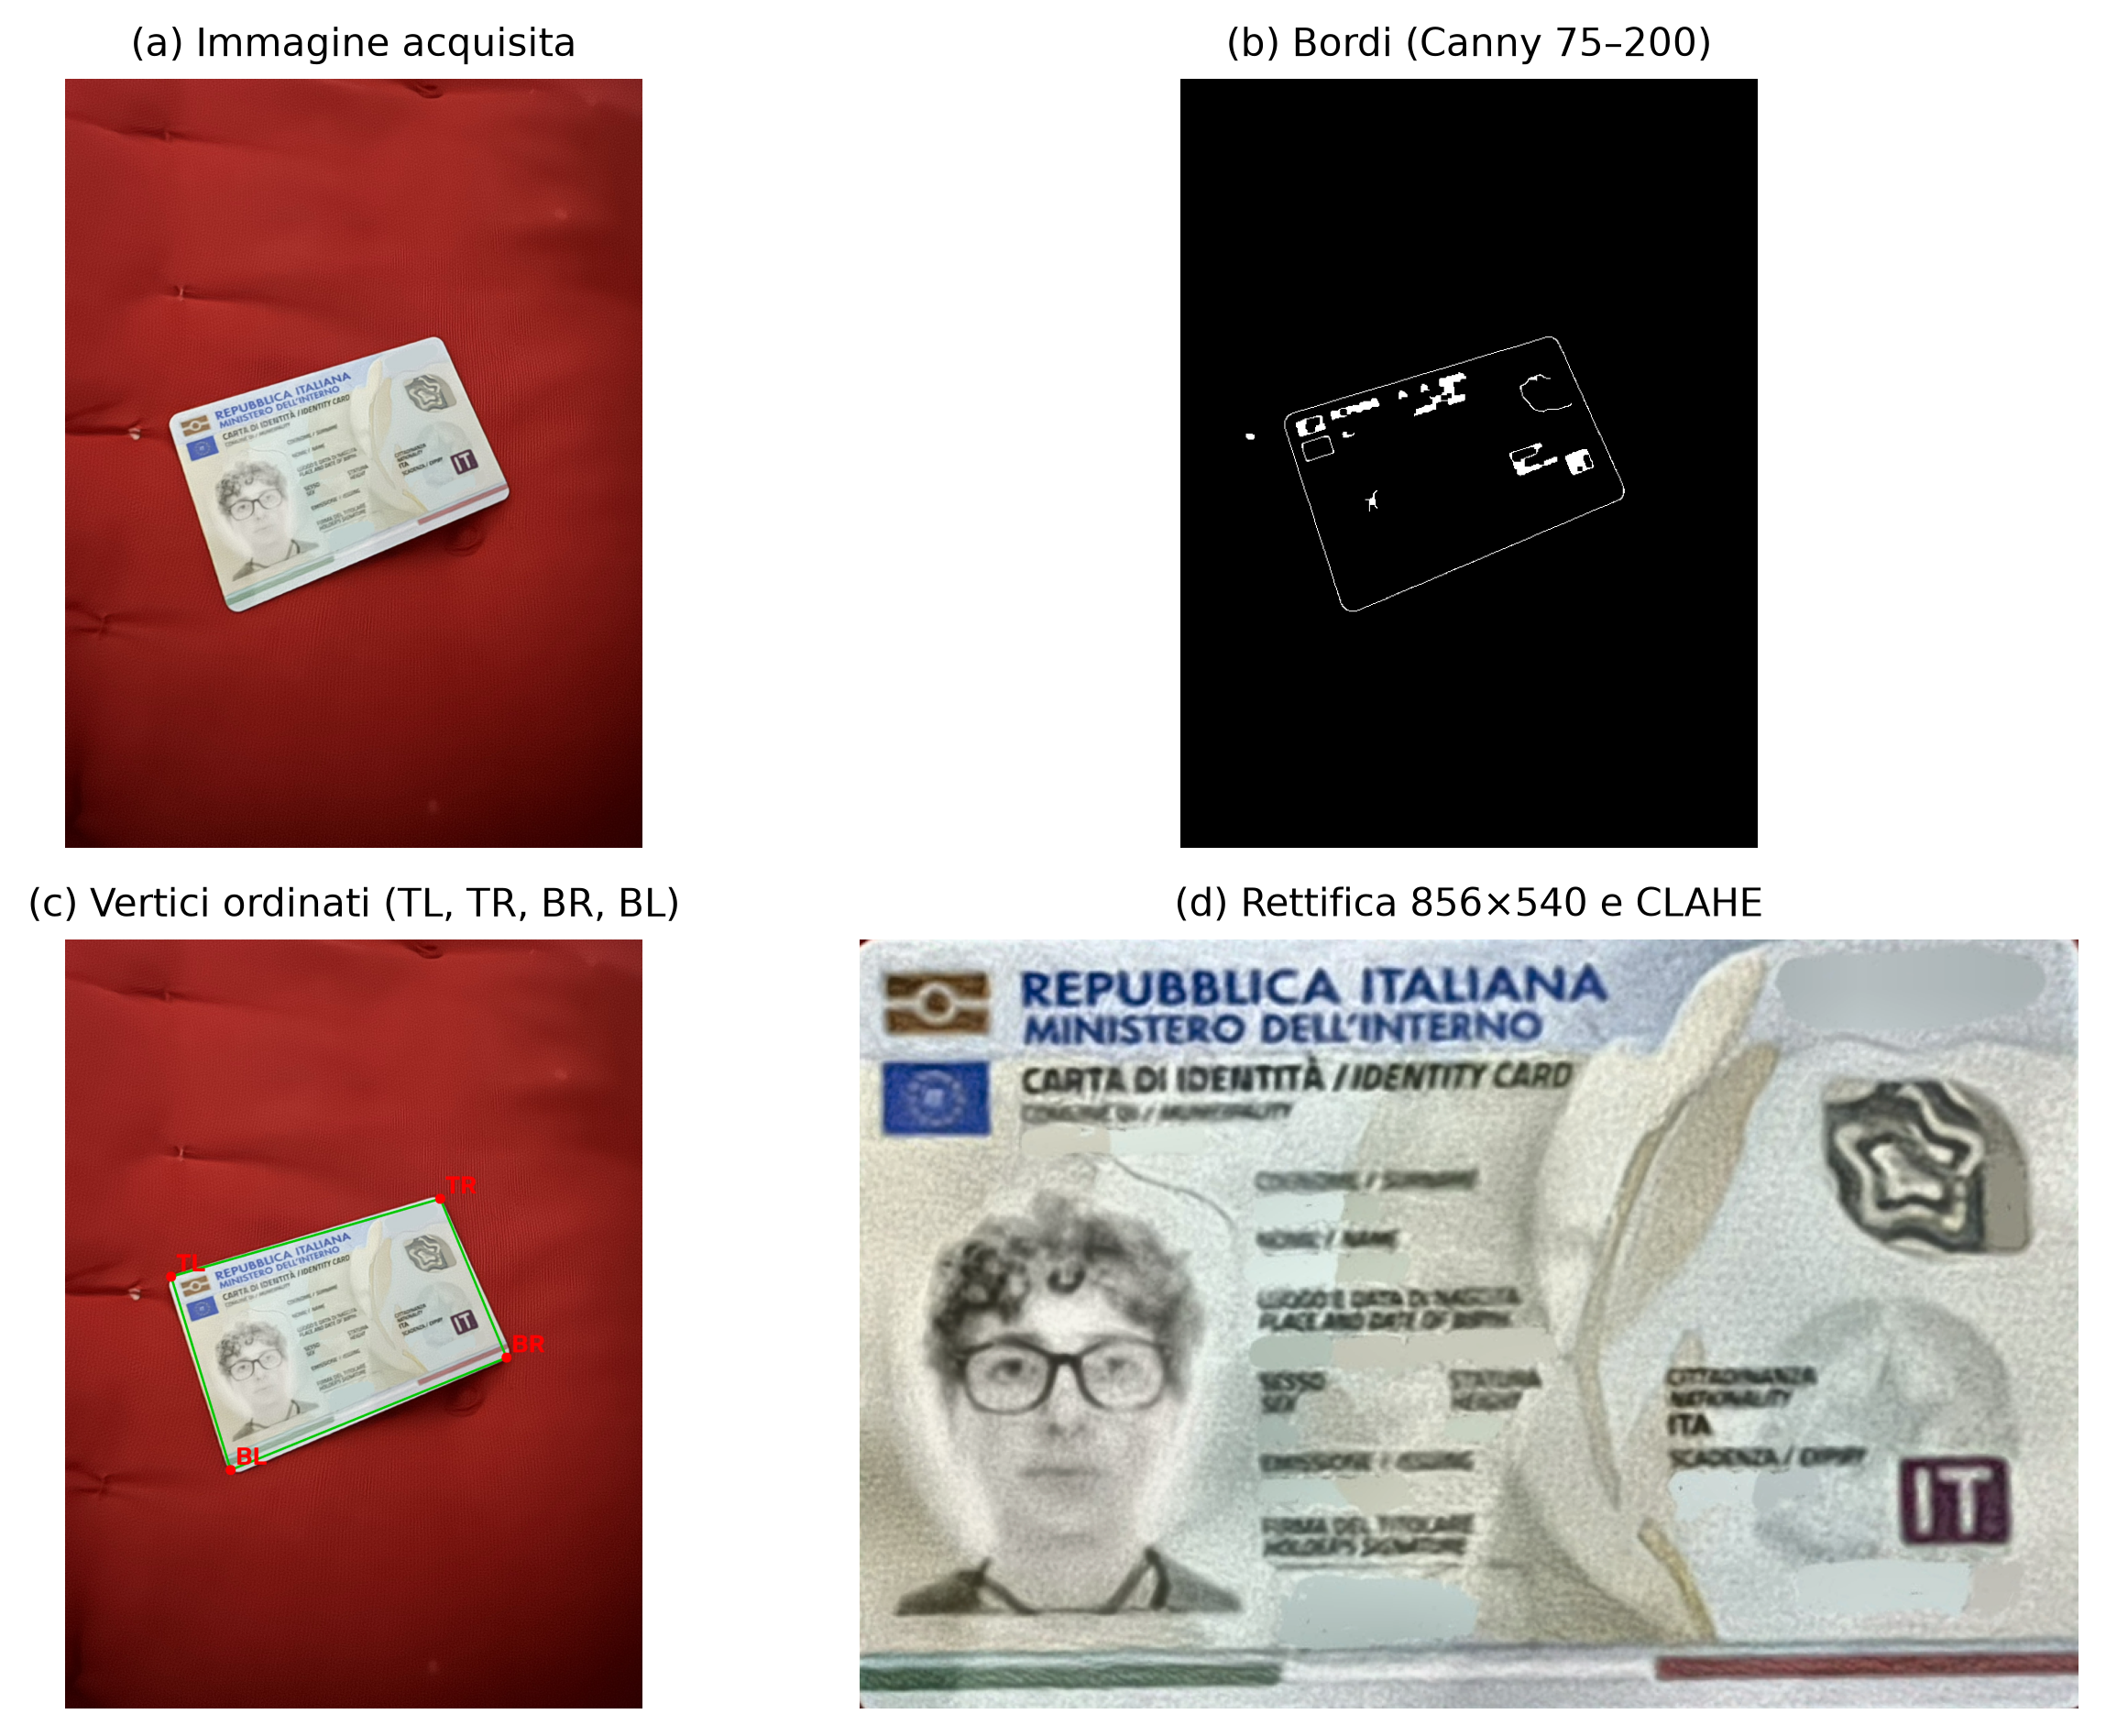
\includegraphics[width=0.9\textwidth]{images/pipeline-cie.png}
    \caption[Fasi della pipeline di rettifica su una \gls{cie} fotografata in ambiente non controllato]{Fasi della pipeline di rettifica su una \gls{cie} fotografata in ambiente non controllato:~(a) immagine acquisita,~(b) bordi estratti,~(c) quadrilatero individuato con i vertici ordinati,~(d) risultato dopo la rettifica a $856 \times 540$ pixel e l'equalizzazione \gls{clahe}. I dati personali sono stati oscurati.}
    \label{fig:pipelineCIE}
\end{figure}
\paragraph{Individuazione della tessera}
La prima versione del modulo cercava il contorno della carta con un'unica combinazione di filtro gaussiano e algoritmo di Canny, e la rettifica falliva sulla maggior parte delle fotografie reali: le venature di un tavolo producevano bordi spuri, mentre un bordo poco contrastato rispetto allo sfondo lasciava il contorno della carta aperto.
La versione attuale affronta i due problemi con quattro accorgimenti:
\begin{itemize}
     \item \textbf{Riduzione della risoluzione}: l'immagine viene ridimensionata in modo che il lato maggiore non superi $800$ pixel. In questo modo i parametri dei filtri hanno lo stesso effetto indipendentemente dalla risoluzione della fotocamera. Le coordinate dei vertici vengono poi riportate alla scala originale.
    \item \textbf{Due tentativi di estrazione dei bordi}, riportati nel Listato~\ref{lst:findCardContour}: \begin{itemize}
    \item Il primo usa un \textbf{filtro bilaterale}, che attenua i pixel vicini nello spazio solo se sono anche simili per intensità, così da levigare le zone omogenee eliminando le texture fini dello sfondo, lasciando nitidi i contorni~\cite{tomasiBilateralFilteringGray1998}.
    \item Se il primo tentativo non produce un contorno valido, si ripete la ricerca con il tradizionale \textbf{filtro gaussiano}, che invece sfoca anche i bordi~\cite{tomasiBilateralFilteringGray1998}. Funziona meglio con le foto delle \gls{cie} dove i contorni sono poco contrastati.
    \end{itemize} 
    In entrambi i casi, si applica il \textit{rilevatore di Canny} seguito da una chiusura morfologica per unire eventuali interruzioni nei bordi.
    \item \textbf{Ricerca del quadrilatero}: sui contorni più estesi, si calcola l'\textit{inviluppo convesso}, che chiude il contorno e ignora le rientranze dovute ad eventuali dita. Il contorno viene poi approssimato con l'algoritmo di \textit{Douglas-Peucker} aumentando gradualmente la tolleranza finché non restano quattro vertici, eliminando anche i punti extra dovuti agli angoli arrotondati della tessera.
    \item \textbf{Validazione geometrica}: per evitare falsi positivi (come fogli, schermi o bordi del tavolo), il quadrilatero viene accettato solo se rispetta i criteri della Tabella~\ref{tab:validazioneQuadrilatero}.  Il controllo principale verifica che il rapporto d'aspetto corrisponda al formato standard ID-1 ($85{,}6/54{,}0 \approx 1{,}58$)~\cite{icao9303}.
\end{itemize}
\begin{lstlisting}[language=Python, caption={I due tentativi di estrazione dei bordi in \texttt{findCardContour} (estratto da \texttt{core/id\_card.py}).}, label={lst:findCardContour}]
attempts = [
    ("bilateral+canny(75,200)", cv2.bilateralFilter(gray, 9, 75, 75), 75, 200),
    ("gaussian+canny(50,150)", cv2.GaussianBlur(gray, (5, 5), 0), 50, 150),
]
for name, smooth, t1, t2 in attempts:
    edged = cv2.Canny(smooth, t1, t2)
    edged = cv2.morphologyEx(edged, cv2.MORPH_CLOSE, np.ones((5, 5), np.uint8))
    target_contour = _detectQuadOnEdges(edged, min_area)
    if target_contour is not None:
        return edged, target_contour.reshape(4, 2).astype("float32") / scale
return edged, None
\end{lstlisting}
\begin{table}[H]
    \centering
    \begin{tabular*}{\textwidth}{@{\extracolsep{\fill}} l l p{6.8cm} @{}}
        \hline
        \textbf{Criterio} & \textbf{Soglia} & \textbf{Motivazione} \\
        \hline
        Area minima & $\ge 10\%$ dell'immagine & Scarta quadrilateri troppo piccoli \\
        Lunghezza dei lati & $\ge 20$ pixel & Esclude poligoni degeneri \\
        Lati opposti & rapporto $\ge 0{,}55$ & Esclude trapezi troppo deformati per essere una carta \\
        Rapporto d'aspetto & $[1{,}25;\ 2{,}05]$ & Compatibilità con il formato ID-1 ($\approx 1{,}58$), con tolleranza per la prospettiva \\
        Angoli interni & $[55^\circ;\ 125^\circ]$ & Plausibilità di un rettangolo visto in prospettiva \\
        \hline
    \end{tabular*}
    \caption{Criteri di validazione del quadrilatero candidato in \texttt{isValidCardQuad}. Le tolleranze sono ampie perché la prospettiva deforma il rettangolo della tessera.}
    \label{tab:validazioneQuadrilatero}
\end{table}
Se nessun candidato supera la validazione in nessuno dei due tentativi, la funzione restituisce l'immagine originale con l'indicatore \texttt{False}: la pipeline prosegue \textbf{senza rettifica} anziché rifiutare la registrazione.
L'approccio adottato si differenzia da quello di sistemi più recenti, che individuano i quattro angoli con una rete neurale \textit{stacked hourglass}, capace di stimarne la posizione anche quando sono occlusi o esterni all'inquadratura~\cite{groteImageQualityAssessment2026}.
Il metodo classico non richiede alcun modello addestrato né dati di documenti reali, la cui disponibilità è limitata da vincoli di \textit{privacy}~\cite{groteImageQualityAssessment2026}. Presuppone che i quattro bordi della tessera siano visibili e le \textbf{conseguenze di questo limite} sono discusse nel Capitolo~\ref{cap:4-risultati}. Per ridurne l'impatto, in~\ref{cap:3.4-ui} si è scelto di guidare l'utente con un'interfaccia che lo aiuti a inquadrare correttamente la tessera.

\paragraph{Ordinamento dei vertici e omografia}
Prima di calcolare la trasformazione prospettica, i quattro vertici devono essere associati agli angoli corretti del rettangolo di destinazione.
La funzione \texttt{orderPoints} li ordina in senso orario in base all'angolo che ciascuno forma con il \textbf{baricentro} del quadrilatero, sceglie come primo vertice quello superiore sinistro e, se necessario, ruota l'ordine in modo che il primo lato sia il lato lungo della tessera, imponendo così l'\textbf{orientamento orizzontale} del formato ID-1.
A differenza di un ordinamento basato sulle sole coordinate, questo criterio resta corretto anche quando la carta è fotografata ruotata, ma essendo completamente geometrico, non considera il contenuto della tessera: una carta capovolta viene invece rettificata capovolta.

Poichè l'acquisizione tramite fotocamera avviene quasi sempre con una certa inclinazione rispetto al piano del documento, la tessera rettangolare appare come un \textbf{trapezio}. Questa deformazione è descritta da una \textbf{trasformazione proiettiva} (omografia)~\cite{thongkorDigitalImageWatermarking2012a}, che in coordinate omogenee si esprime come specificato nell'Equazione~\eqref{eq:omografia}:
\begin{equation}
    \label{eq:omografia}
    \begin{bmatrix} X_p & Y_p & Z_p \end{bmatrix} =
    \begin{bmatrix} x & y & 1 \end{bmatrix}
    \begin{bmatrix} a & d & g \\ b & e & h \\ c & f & 1 \end{bmatrix},
    \qquad
    X = \frac{X_p}{Z_p}, \quad Y = \frac{Y_p}{Z_p}
\end{equation}
dove $(x,y)$ è un punto dell'immagine acquisita e $(X,Y)$ il punto corrispondente nell'immagine rettificata.
Gli otto parametri $a, \dots, h$ vengono determinati da quattro coppie di punti di controllo~\cite{thongkorDigitalImageWatermarking2012a} che coincidono con i vertici individuati, associati agli angoli del rettangolo di destinazione, come mostrato anche in Figura~\ref{fig:pipelineCIE}:
\begin{itemize} 
    \item$(0,0)\rightarrow\text{angolo superiore sinistro (TL)}$, 
    \item$(W-1,0)\rightarrow\text{angolo superiore destro (TR)}$, 
    \item$(W-1,H-1)\rightarrow\text{angolo inferiore destro (BR)}$ 
    \item$(0,H-1)\rightarrow\text{angolo inferiore sinistro (BL)}$.
\end{itemize}
\begin{lstlisting}[language=Python, caption={Calcolo dell'omografia e rettifica in \texttt{fixProspective} (estratto da \texttt{core/id\_card.py}).}, label={lst:omografia}]
rect = orderPoints(punti)
out_w, out_h = targetSize
out_pts = np.array([[0, 0], [out_w - 1, 0],
                    [out_w - 1, out_h - 1], [0, out_h - 1]], dtype="float32")
matrix = cv2.getPerspectiveTransform(rect, out_pts)
fixedImage = cv2.warpPerspective(original, matrix, targetSize)
\end{lstlisting}
La funzione \texttt{getPerspectiveTransform} nel Listato~\ref{lst:omografia}  calcola la matrice $3 \times 3$ a partire dalle quattro corrispondenze, e \texttt{warpPerspective} la applica all'immagine originale a piena risoluzione~\cite{OpenCV-docs}.
Le dimensioni di destinazione $W \times H = 856 \times 540$ pixel corrispondono al formato ID-1 di $85{,}6 \times 54{,}0~\text{mm}$ in scala di dieci pixel per millimetro, e ne preservano il rapporto d'aspetto~\cite{icao9303}.

\paragraph{Equalizzazione del contrasto}
La funzione \texttt{enhanceContrast} applica \gls{clahe} operando esclusivamente sulla luminanza (Listato~\ref{lst:enhanceContrast}).

\begin{lstlisting}[language=Python, caption={Equalizzazione CLAHE sul canale di luminanza (estratto da \texttt{core/id\_card.py}).}, label={lst:enhanceContrast}]
lab = cv2.cvtColor(image, cv2.COLOR_BGR2LAB)
l_channel, a_channel, b_channel = cv2.split(lab)
clahe = cv2.createCLAHE(clipLimit=2.0, tileGridSize=(8, 8))
l_enhanced = clahe.apply(l_channel)
lab_enhanced = cv2.merge([l_enhanced, a_channel, b_channel])
return cv2.cvtColor(lab_enhanced, cv2.COLOR_LAB2BGR)
\end{lstlisting}
L'immagine è convertita nello \textbf{spazio LAB}, che separa la luminanza $L$ dalle componenti cromatiche $a$ e $b$. In questo modo si può equalizzare il solo canale $L$, aumentando il contrasto senza alterare le tonalità.
Una classica equalizzazione globale applica la stessa correzione a tutta l'immagine, risultando inefficace quando l'illuminazione non è uniforme~\cite{rezaRealizationContrastLimited2004}, che risulta essere un problema frequente sui documenti in policarbonato, spesso soggetti a riflessi localizzati. 
Per superare questo limite si utilizza \gls{clahe}, che opera in tre fasi~\cite{rezaRealizationContrastLimited2004}:
\begin{enumerate}
    \item suddivide l'immagine in una griglia e calcola una mappatura locale per ciascun riquadro;
    \item limita l'amplificazione del contrasto per evitare di accentuare il rumore nelle aree uniformi;
    \item fonde i confini tra riquadri adiacenti tramite \textit{interpolazione bilineare}, eliminando l'effetto a blocchi.
\end{enumerate}
Nel sistema la griglia è di $8 \times 8$ regioni, la stessa suddivisione indicata in letteratura per una buona stima statistica degli istogrammi locali~\cite{rezaRealizationContrastLimited2004}. Invece il limite di contrasto è fissato a $2{,}0$~\cite{rezaRealizationContrastLimited2004}. L'effetto di \gls{clahe} sul \textit{matching} è valutato nel Capitolo~\ref{cap:4-risultati}.
La Figura~\ref{fig:istogrammiClahe} mostra come l'equalizzazione allarghi la distribuzione della luminanza dell'immagine rettificata.
\begin{figure}[H]
    \centering
    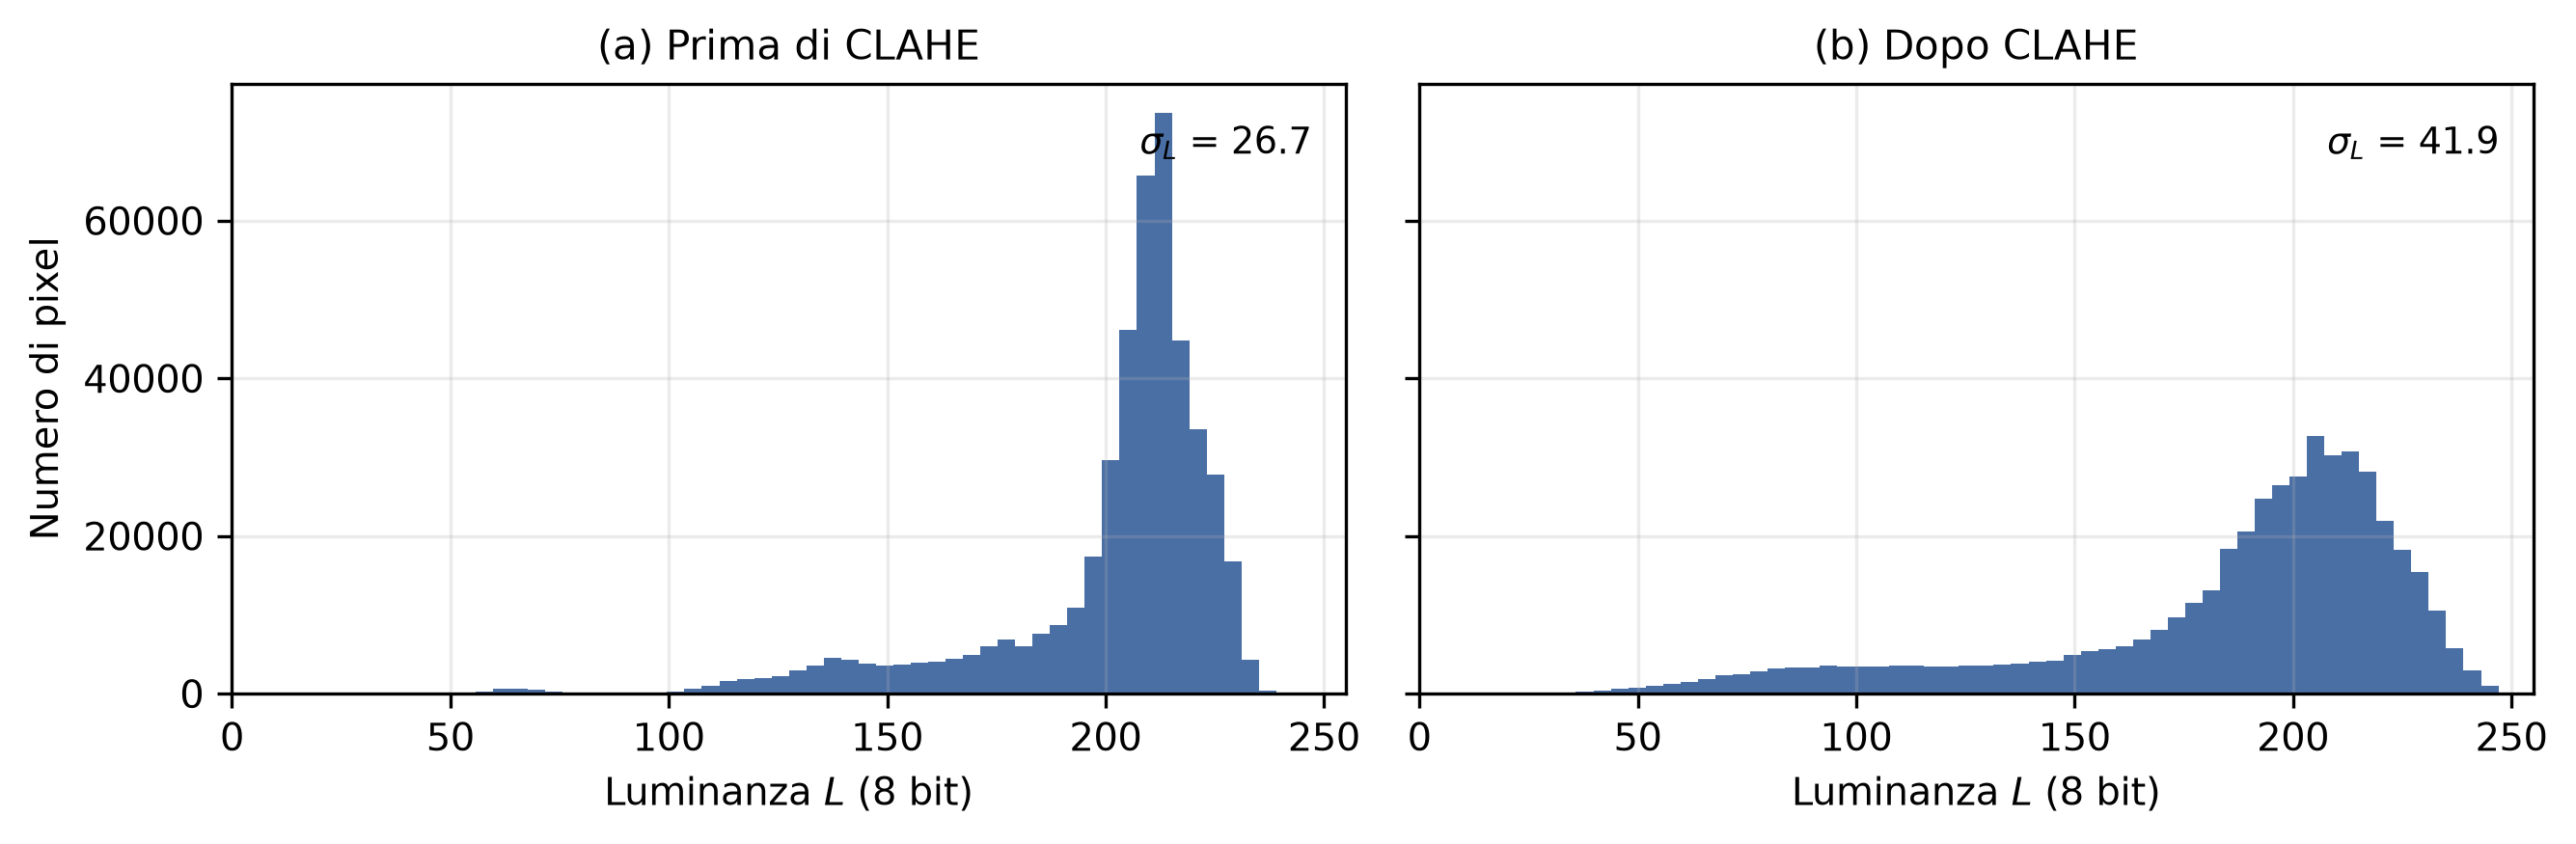
\includegraphics[width=\textwidth]{images/istogrammi-clahe.png}
    \caption[Istogramma della luminanza $L$ della \gls{cie} rettificata]{Istogramma della luminanza $L$ della \gls{cie} rettificata prima (a) e dopo (b) l'equalizzazione \gls{clahe}. $\sigma_L$ indica la deviazione standard della luminanza.}
    \label{fig:istogrammiClahe}
\end{figure}
\paragraph{Composizione della pipeline}
La funzione \texttt{preprocessIDCard} applica in sequenza la rettifica e l'equalizzazione, restituendo insieme all'immagine un dizionario di indicatori (\texttt{fixes}) che registra quali correzioni sono state effettivamente applicate.
Eseguendo l'equalizzazione dopo la rettifica, gli istogrammi locali vengono calcolati sulla sola superficie della tessera, senza che lo sfondo ne influenzi la distribuzione.
Se invece la rettifica non riesce, \gls{clahe} viene comunque applicato all'immagine originale, poiché migliora la leggibilità del volto indipendentemente dalla geometria.
Gli indicatori sono restituiti al client nei campi \texttt{fixProspective} e \texttt{fixContrast} del contratto di risposta all'\textit{enrollment} (Capitolo~\ref{cap:2.4.2-modelloDati}), così che l'interfaccia possa segnalare se il documento è stato raddrizzato.
L'immagine così normalizzata viene infine consegnata alla stessa funzione di rilevamento della \textit{live verification} (Capitolo~\ref{cap:3.2.2-faceAnalysis}).
La volto del documento e il volto ripreso dalla fotocamera seguono quindi un unico percorso di allineamento ed estrazione, condizione necessaria affinchè i due embedding siano confrontabili.

\subsection{Rilevamento, allineamento ed estrazione con InsightFace}\label{cap:3.2.2-faceAnalysis}
Il confronto tra il ritratto della \gls{cie} e il volto ripreso dalla fotocamera ha senso solo se le due immagini attraversano lo stesso percorso di elaborazione. 
Un rilevatore diverso o un allineamento diverso sposterebbero gli embedding in regioni differenti dello spazio vettoriale, indipendentemente dall'identità.
Per questo il sistema usa un'unica funzione, \texttt{pipelineFaceDetection}, sia nell'\textit{enrollment} sia in ogni fotogramma della \textit{live verification}, appoggiandosi alla libreria \textit{InsightFace}~\cite{github-insightface}.

\paragraph{Il pacchetto \texttt{buffalo\_l}}
\textit{InsightFace} distribuisce i propri modelli in pacchetti già esportati in formato \gls{onnx}, e la classe \texttt{FaceAnalysis} utilizza per impostazione predefinita il pacchetto \texttt{buffalo\_l}~\cite{github-insightface}.
Il pacchetto contiene cinque grafi distinti, riportati nella Tabella~\ref{tab:buffaloL}: il sistema ne carica soltanto due, indicandoli nel parametro \texttt{allowed\_modules}, perché i landmark densi e la stima di genere ed età non servono alla verifica dell'identità e occuperebbero memoria e tempo di inferenza a ogni fotogramma.

\begin{table}[H]
    \centering
    \footnotesize
    \renewcommand{\arraystretch}{1.25}
    \begin{tabular*}{\textwidth}{@{\extracolsep{\fill}} >{\raggedright\arraybackslash}p{2.6cm} >{\raggedright\arraybackslash}p{3.4cm} >{\raggedright\arraybackslash}p{6.0cm} c @{}}
        \hline
        \textbf{File} & \textbf{Modello} & \textbf{Funzione} & \textbf{Caricato} \\
        \hline
        \texttt{det\_10g.onnx} & SCRFD-10GF & Rilevamento del volto, \textit{bounding box} e 5 keypoint & Sì \\
        \texttt{w600k\_r50.onnx} & ResNet-50 su WebFace600K & Estrazione dell'embedding a 512 dimensioni & Sì \\
        \texttt{2d106det.onnx} & Landmark 2D & 106 punti di riferimento del volto & No \\
        \texttt{1k3d68.onnx} & Landmark 3D & 68 punti di riferimento tridimensionali & No \\
        \texttt{genderage.onnx} & Attributi & Stima di genere ed età & No \\
        \hline
    \end{tabular*}
    \caption{Composizione del pacchetto \texttt{buffalo\_l} di \textit{InsightFace} e moduli effettivamente caricati dal sistema~\cite{github-insightface}.}
    \label{tab:buffaloL}
\end{table}
L'inizializzazione, riportata nel Listato~\ref{lst:initFaceRecognition}, avviene una sola volta all'avvio del server (Capitolo~\ref{cap:3.3-orchestrazione}).
Il valore \texttt{ctx\_id=-1} forza l'esecuzione su CPU, per il \textit{deployment} senza acceleratori grafici.

\begin{lstlisting}[float=h, language=Python, caption={Inizializzazione del modulo di analisi facciale (\texttt{core/face\_detector.py}).}, label={lst:initFaceRecognition}]
def initFaceRecognition(model: str = "buffalo_l",
                        det_size: tuple[int, int] = (320, 320)) -> FaceAnalysis:
    app = FaceAnalysis(name=model, root="../.insightface",
                       allowed_modules=['detection', 'recognition'])
    app.prepare(ctx_id=-1, det_size=det_size)
    return app
\end{lstlisting}

\paragraph{Rilevamento e risoluzione di ingresso}
Il rilevatore incluso in \texttt{buffalo\_l} appartiene alla famiglia \textit{\gls{scrfd}}, progettata per bilanciare \textbf{precisione e velocità di calcolo}~\cite{guoSampleComputationRedistribution2021}. 
Il modello analizza l'immagine su tre diverse scale per individuare sia volti piccoli e lontani sia primi piani~\cite{guoSampleComputationRedistribution2021}.
La versione distribuita da \textit{InsightFace} individua contemporaneamente il riquadro del volto e i 5 \textit{punti chiave} (occhi, naso e angoli della bocca)~\cite{github-insightface}, senza dover caricare un secondo modello dedicato.

Il parametro \texttt{det\_size} $= (320, 320)$ imposta la risoluzione a cui viene ridimensionata l'immagine prima di cercare il volto. 
Questa scelta si adatta bene al contesto applicativo: a differenza dei benchmark generici dominati da volti molto piccoli (inferiori a $32 \times 32$ pixel)~\cite{guoSampleComputationRedistribution2021}, sia nel selfie sia nel documento rettificato il viso occupa gran parte dell'inquadratura. 
Ridurre la risoluzione a $320 \times 320$ pixel non compromette quindi il rilevamento, ma abbassa sensibilmente il carico di calcolo su ogni fotogramma del buffer.

\paragraph{Selezione del volto principale}
Il metodo \texttt{FaceAnalysis.get} restituisce una lista di oggetti, uno per ogni volto rilevato, ciascuno con:
\begin{itemize}
    \item il riquadro \texttt{bbox} $=(x_1, y_1, x_2, y_2)$, 
    \item la confidenza di rilevamento \texttt{det\_score},
    \item i keypoint \texttt{kps},
    \item l'embedding \texttt{embedding}.
\end{itemize}
Poiché l'immagine può contenere più volti, la funzione \texttt{getMainFace} sceglie come soggetto il volto con il riquadro di area massima, secondo l'Equazione~\eqref{eq:voltoPrincipale}:
\begin{equation}
    \label{eq:voltoPrincipale}
    f^{*} = \arg\max_{f \in \mathcal{F}} \; \big(x_2^{(f)} - x_1^{(f)}\big)\,\big(y_2^{(f)} - y_1^{(f)}\big)
\end{equation}
dove $\mathcal{F}$ è l'insieme dei volti rilevati nell'immagine.
Il criterio dell'area, a differenza di quello della confidenza, privilegia il soggetto più vicino alla fotocamera, che coincide con l'utente che si sta autenticando.
Il Listato~\ref{lst:pipelineFaceDetection} mostra la composizione delle due operazioni.\\
Quando nessun volto viene rilevato, la funzione restituisce \texttt{None}, condizione che l'\textit{endpoint} di registrazione traduce in un errore e il canale WebSocket nello stato \texttt{WAITING\_FACE}.

\begin{lstlisting}[float=htbp,language=Python, caption={Rilevamento e selezione del volto principale (\texttt{core/face\_detector.py}).}, label={lst:pipelineFaceDetection}]
def getMainFace(faces: list):
    if not faces:
        return None
    return max(faces, key=lambda face:
               (face.bbox[2]-face.bbox[0]) * (face.bbox[3]-face.bbox[1]))

def pipelineFaceDetection(detector: FaceAnalysis, image: np.ndarray):
    faces = getFaces(detector, image)
    mainFace = getMainFace(faces)
    if mainFace is None:
        return None, image
    return mainFace
\end{lstlisting}

\paragraph{Allineamento ed estrazione dell'embedding}
L'allineamento sui 5 keypoint e il ritaglio a $112 \times 112$ pixel, descritti nel Capitolo~\ref{cap:1.1-fondamenti}, rispecchiano la pre-elaborazione standard con cui \gls{arcface} viene addestrata e valutata.
Nel pacchetto \texttt{buffalo\_l}, il modello si basa su una rete \textit{ResNet-50} addestrata su \textit{WebFace600K}~\cite{github-insightface}.
Rispetto alla variante più pesante \textit{ResNet-100}, riduce l'occupazione in memoria (circa 160~MB contro 250~MB) e quasi dimezza i tempi di estrazione ($8{,}9$~ms contro $15{,}4$~ms per volto)~\cite{dengArcFaceAdditiveAngular2022}.
La funzione \texttt{extractEmbeddings} nel Listato~\ref{lst:verifyIdentity} estrae quindi la confidenza di rilevamento e copia il vettore prodotto dalla rete per svincolarlo dalle strutture interne della libreria. 
\begin{figure}[H]
    \centering
    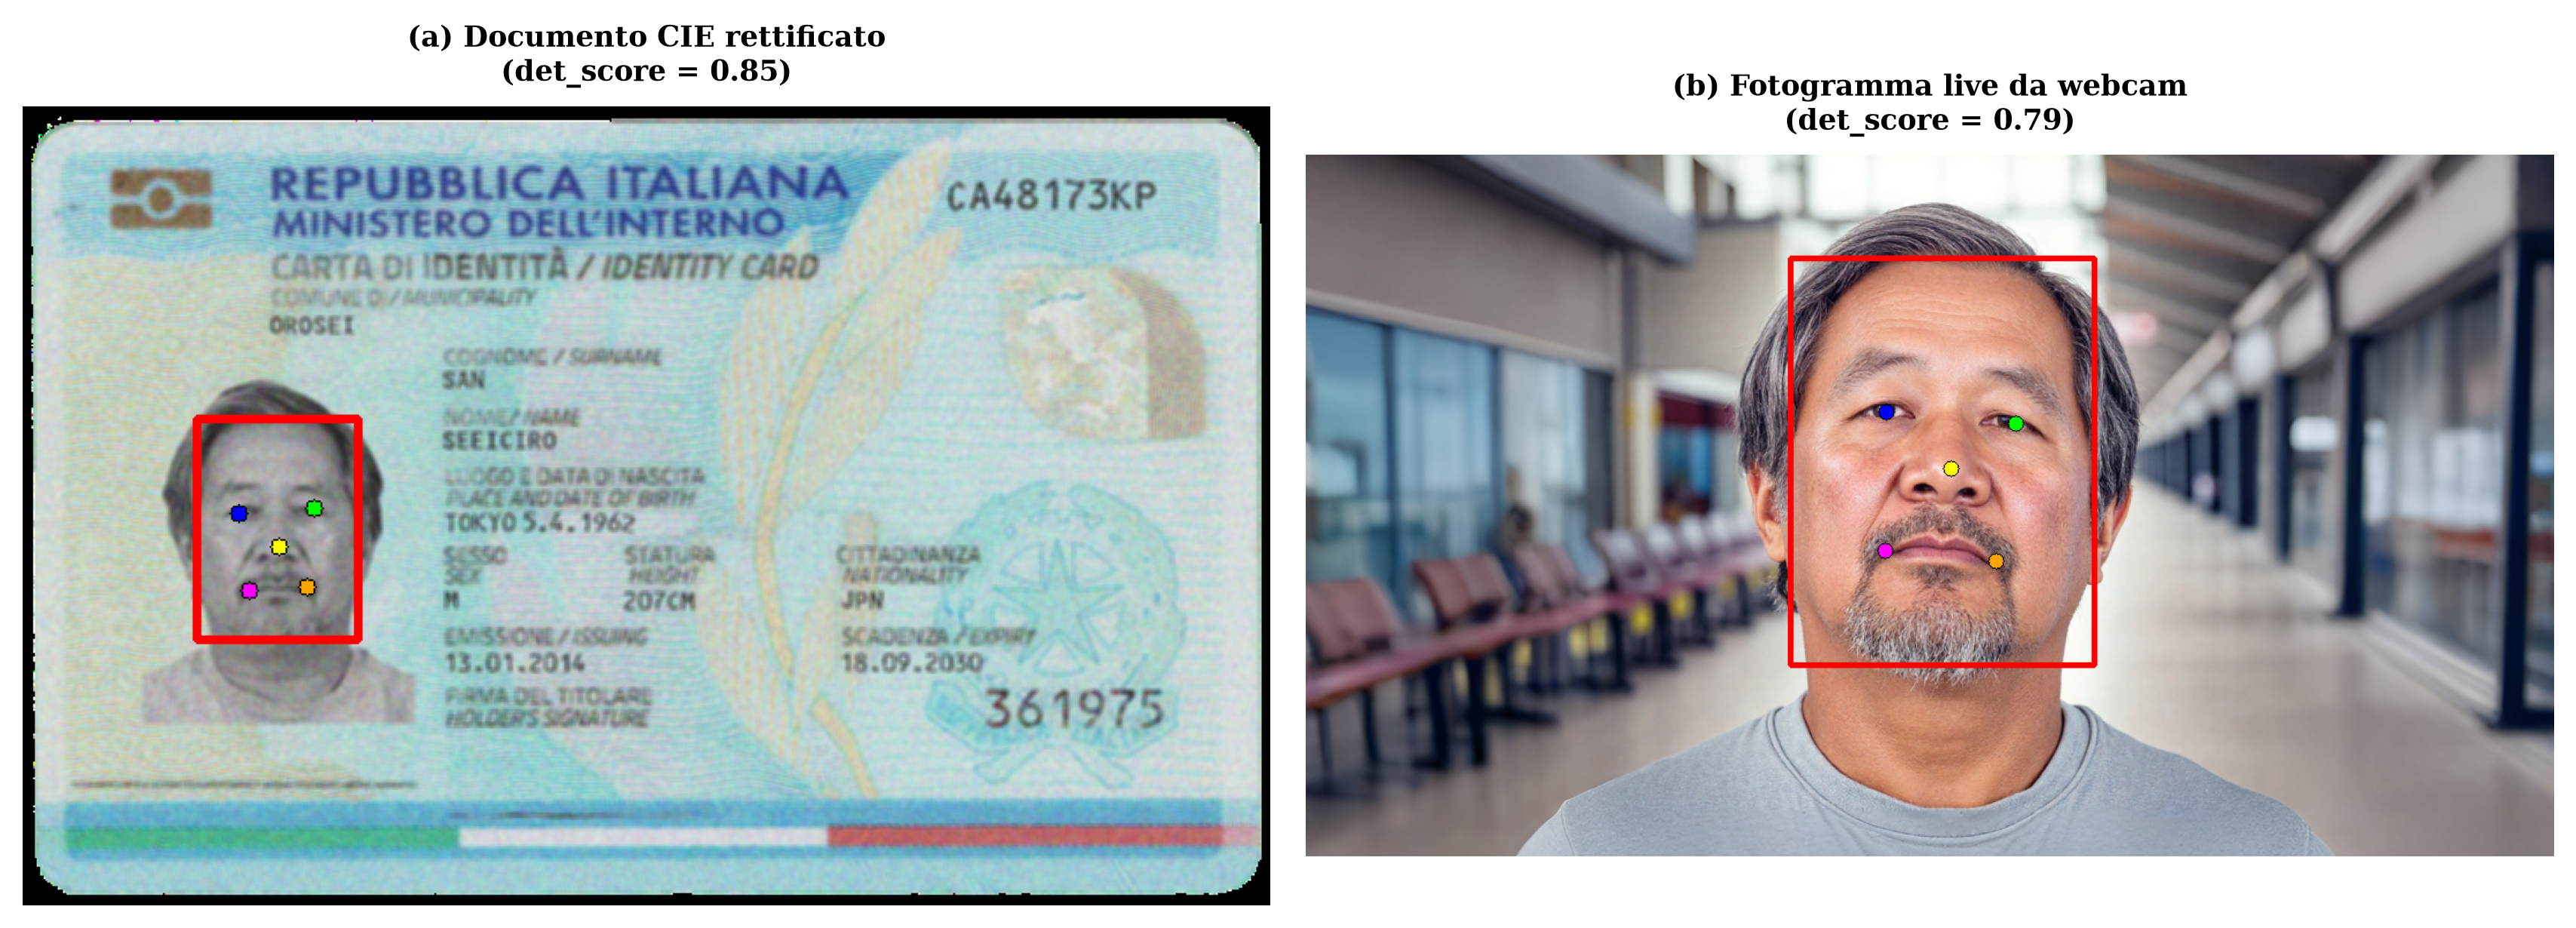
\includegraphics[width=0.95\textwidth]{images/confronto_bbox_kps.png}
    \caption[Output del modulo di rilevamento facciale]{Output del modulo di rilevamento facciale sul ritratto della \gls{cie} rettificata (a) e su un fotogramma acquisito in diretta (b), con evidenza del \textit{bounding box} e dei 5 \textit{keypoint} biometrici utilizzati per l'allineamento affine a $112 \times 112$ pixel.}
    \label{fig:confrontoBboxKps}
\end{figure}
\paragraph{Verifica tramite similarità coseno}
\gls{arcface} distribuisce i vettori su un'ipersfera, come descritto nel Capitolo~\ref{cap:1-fondamenti}.
Il confronto, quindi, avviene tramite la similarità coseno dell'Equazione~\eqref{eq:cosineSimilarity}.
L'implementazione, riportata nel Listato~\ref{lst:verifyIdentity}, calcola il rapporto tra il prodotto scalare dei due vettori e il prodotto delle rispettive norme.
Poichè i vettori in ingresso non sono normalizzati, restituisce $0$ quando uno dei due vettori manca o ha norma nulla, evitando una divisione per zero.

\begin{lstlisting}[float=htbp, language=Python, caption={Estrazione dell'embedding e verifica tramite similarit\`a coseno (\texttt{core/face\_recognizer.py})}, label={lst:verifyIdentity}]
def extractEmbeddings(face):
    if face is None or not hasattr(face, 'embedding'):
        return (None, 0.0)
    return face.embedding.copy(), float(face.det_score)

def cosineSimilarity(embedding1: np.ndarray, embedding2: np.ndarray):
    if embedding1 is None or embedding2 is None:
        return 0.0
    dot_product = embedding1 @ embedding2
    norm1 = np.linalg.norm(embedding1)
    norm2 = np.linalg.norm(embedding2)
    if norm1 == 0 or norm2 == 0:
        return 0.0
    return dot_product / (norm1 * norm2)

def verifyIdentity(embedding1, embedding2, threshold=0.45):
    similarity = cosineSimilarity(embedding1, embedding2)
    return {"similarity": float(similarity),
            "isMatch": similarity >= threshold,
            "threshold": float(threshold)}
\end{lstlisting}

La funzione \texttt{verifyIdentity} applica la regola decisionale $S_c \ge \tau$ e restituisce, oltre all'esito, il valore di similarità e la soglia usata, così che il client possa mostrarli.

\subsection{Verifica di vitalità con MiniFASNet su ONNX Runtime}\label{cap:3.2.3-livenessOnnx}
Il modello di \textit{liveness}, viene caricato in formato \gls{onnx} ed eseguito tramite \textit{ONNX Runtime}~\cite{ONNXRuntime}. 
Questo approccio evita di installare l'intero framework di addestramento sul server, riducendo le dipendenze e rendendo il modello portabile su qualsiasi piattaforma senza modifiche.

La rete utilizzata è \textit{MiniFASNetV2}, tratta dal progetto \textit{Silent-Face-Anti-Spoofing}~\cite{MinivisionaiSilentFaceAntiSpoofing}. 
Durante l'addestramento, la rete è affiancata da un ramo ausiliario che analizza lo spettro di Fourier dell'immagine per distinguere un volto reale da una contraffazione~\cite{MinivisionaiSilentFaceAntiSpoofing}: infatti, le foto reali mostrano componenti ad alta frequenza lungo le diagonali ($45^\circ$ e $135^\circ$), mentre le riproduzioni su carta o schermo le concentrano lungo gli assi orizzontale e verticale~\cite{liSilentFaceAntiSpoofing2024}.

Come riportato nella Tabella~\ref{tab:minifasnet}, \textit{MiniFASNetV2} è una versione alleggerita (\textit{pruned}) di \textit{MobileFaceNet} che richiede meno di $0{,}1$ GFLOP e meno di mezzo milione di parametri, risultando ideale per l'esecuzione in tempo reale su CPU.
\begin{table}[H]
    \centering
    \footnotesize
    \renewcommand{\arraystretch}{1.25}
    \begin{tabular*}{\textwidth}{@{\extracolsep{\fill}} l c c @{}}
        \hline
        \textbf{Modello} & \textbf{Complessità [GFLOPs]} & \textbf{Parametri [milioni]} \\
        \hline
        MobileFaceNet & 0,224 & 0,991 \\
        MiniFASNetV1 & 0,081 & 0,414 \\
        MiniFASNetV2 & 0,081 & 0,435 \\
        \hline
    \end{tabular*}
    \caption{Costo computazionale delle reti del progetto \textit{Silent-Face-Anti-Spoofing}~\cite{MinivisionaiSilentFaceAntiSpoofing}.}
    \label{tab:minifasnet}
\end{table}
Il progetto originale~\cite{MinivisionaiSilentFaceAntiSpoofing} prevede l'uso combinato di più modelli addestrati su diverse scale di ritaglio del volto, sommandone le probabilità in uscita per classificare il soggetto come reale~\cite{MinivisionaiSilentFaceAntiSpoofing}. 
L'integrazione con il secondo modello della suite (addestrato a scala $4{,}0$) non è stata inclusa per contenere i tempi di inferenza e viene discussa tra i limiti nel Capitolo~\ref{cap:conclusioni}.

\paragraph{Caricamento della sessione di inferenza.}
La funzione \texttt{loadLivenessModel} (Listato~\ref{lst:livenessModel}) verifica che il file indicato da \texttt{LIVENESS\_MODEL\_PATH} esista, sollevando un errore esplicito in caso contrario, e crea una \texttt{InferenceSession}.
Come per \textit{InsightFace}, la sessione viene creata una sola volta all'avvio e riutilizzata da tutte le connessioni (Capitolo~\ref{cap:3.3-orchestrazione}).

\begin{lstlisting}[float=htbp, language=Python, caption={Caricamento del grafo \gls{onnx} di \textit{MiniFASNetV2} (\texttt{core/liveness.py}).}, label={lst:livenessModel}]
def loadLivenessModel(modelPath: str):
    if not os.path.exists(modelPath):
        raise FileNotFoundError(f"Modello MiniFASNet non trovato: {modelPath}")
    return ort.InferenceSession(modelPath,
                                providers=["CPUExecutionProvider"])
\end{lstlisting}

\paragraph{Ritaglio con contesto}
A differenza del modulo di riconoscimento, che lavora sul solo volto allineato, il classificatore di vitalità necessita un ritaglio \textbf{più ampio} del riquadro di rilevamento, che include anche una parte della scena attorno al volto.
La funzione \texttt{scaleBbox} riproduce il calcolo del progetto originale~\cite{MinivisionaiSilentFaceAntiSpoofing}, adattandolo al formato $(x_1, y_1, x_2, y_2)$ dei riquadri di \textit{InsightFace}.
Dato un riquadro di dimensioni $w \times h$ e centro $(c_x, c_y)$ in un'immagine di $W \times H$ pixel, il fattore di scala effettivo viene limitato in modo che il ritaglio non superi le dimensioni dell'immagine, come descritto nell'Equazione~\eqref{eq:scalaRitaglio}:
\begin{equation}
    \label{eq:scalaRitaglio}
    s^{*} = \min\left( s, \; \frac{H-1}{h}, \; \frac{W-1}{w} \right), \qquad s = 2{,}7
\end{equation}
Il nuovo riquadro ha dimensioni $s^{*}w \times s^{*}h$ ed è centrato in $(c_x, c_y)$.
Se esce dall'immagine su un lato, viene traslato verso l'interno della quantità eccedente, mantenendone invariate le dimensioni.
In questo modo il volto resta al centro del ritaglio quando è lontano dai bordi, mentre per un volto vicino al bordo viene sacrificata la centratura e non la quantità di contesto.
Il ritaglio è infine ridimensionato a $80 \times 80$ pixel, la dimensione di ingresso del modello.

\paragraph{Inferenza e normalizzazione delle uscite}
La funzione \texttt{predictLiveness} (Listato~\ref{lst:predictLiveness}) prepara il ritaglio per il modello trasformandolo in un tensore \texttt{float32} di dimensione $(1, 3, 80, 80)$. 
L'operazione riorganizza gli assi dal formato \textit{OpenCV} (altezza, larghezza, canali: HWC) a quello richiesto dalle reti \textit{PyTorch} (canali, altezza, larghezza: CHW), aggiungendo infine la dimensione del \textit{batch} (un immagine alla volta).
Come nel progetto originale~\cite{MinivisionaiSilentFaceAntiSpoofing}, i canali restano nell'ordine BGR (Blu-Verde-Rosso)\footnote{Gli autori hanno addestrato il modello con questa scala non normalizzata, quindi alterarla falserebbe la distribuzione degli ingressi, rendendo inaffidabili le predizioni del modello.} e i valori dei pixel vengono mantenuti nell'intervallo $[0, 255]$ senza normalizzazione.

\begin{lstlisting}[float=htbp, language=Python, caption={Inferenza di \textit{MiniFASNetV2} e softmax numericamente stabile (\texttt{core/liveness.py}).}, label={lst:predictLiveness}]
def predictLiveness(session: ort.InferenceSession, crop_bgr: np.ndarray):
    blob = crop_bgr.astype(np.float32)        # uint8 -> float32
    blob = np.transpose(blob, (2, 0, 1))      # HWC -> CHW
    blob = np.expand_dims(blob, axis=0)       # batch (1, 3, 80, 80)

    outputs = session.run(None, {"input": blob})
    logits = np.array(outputs[0])[0] #Risposta rete grezza

    exp_l = np.exp(logits - np.max(logits))   # softmax stabile
    probs = exp_l / np.sum(exp_l)
    return float(probs[1]), float(probs[0]), float(probs[2])  
    # real, print, screen
\end{lstlisting}

Il grafo restituisce tre valori non normalizzati (\textit{logit}) $z_0, z_1, z_2$, uno per classe.
Le probabilità si ottengono con la funzione \textbf{\textit{softmax}}, calcolata nella forma numericamente stabile dell'Equazione~\eqref{eq:softmaxStabile}:
\begin{equation}
    \label{eq:softmaxStabile}
    p_k = \frac{e^{\,z_k - z_{\max}}}{\sum_{j=0}^{2} e^{\,z_j - z_{\max}}}, \qquad z_{\max} = \max_j z_j, \quad k \in \{0, 1, 2\}
\end{equation}
Sottrarre $z_{\max}$ a tutti i logit non cambia il risultato, perché il fattore $e^{-z_{\max}}$ compare sia al numeratore sia al denominatore, ma garantisce che tutti gli esponenti siano minori o uguali a zero. Il termine più grande vale esattamente $1$ (percentuale massima), così che nessun esponenziale può superare il limite di rappresentazione dei numeri in virgola mobile.

\paragraph{Regola di decisione sul singolo fotogramma}
La funzione \texttt{checkLiveness} compone le operazioni precedenti e classifica il fotogramma come genuino secondo l'Equazione~\eqref{eq:decisioneFrame}:
\begin{equation}
    \label{eq:decisioneFrame}
    \text{live}(f_t) \iff p_{\text{real}} \ge \tau_{\text{liveness}} \;\land\; p_{\text{real}} > p_{\text{print}} \;\land\; p_{\text{real}} > p_{\text{screen}}
\end{equation}
Se il fotogramma non è genuino, il tipo di attacco riportato è la classe di attacco più probabile tra \texttt{PRINT} e \texttt{SCREEN}.
Se il ritaglio fallisce, la funzione restituisce uno \textit{score} nullo e il tipo \texttt{CROP FAILED}, così che il fotogramma sia trattato come non genuino invece di interrompere la sessione.
Il risultato della funzione contiene lo \textit{score} $p_{\text{real}}$, il tipo di attacco, le tre probabilità e la soglia applicata.
% Detection, keypoints ed estrazione embedding con InsightFace; Verifica coseno; Inferenza multi-scala MiniFASNet su ONNX Runtime
% 7pp
\section{Orchestrazione REST, WebSocket e Database}\label{cap:3.3-orchestrazione}
Il compito di trasformare i moduli biometrici descritti nel Capitolo~\ref{cap:3.2-moduliBiometrici} in un servizio spetta al \textbf{livello di orchestrazione}, che deve risolvere tre problemi: caricare i modelli una sola volta e condividerli tra tutte le richieste, verificare ogni dato in ingresso prima che raggiunga una rete neurale e infine tradurre la \gls{fsm} del Capitolo~\ref{cap:2.3-pipeline} in un ciclo di ricezione e risposta su WebSocket, chiuso da un'unica interrogazione al database.

\paragraph{Ciclo di vita del server}
\textit{FastAPI} permette di associare all'applicazione una funzione di ciclo di vita (\textit{lifespan}): il codice che precede l'istruzione \texttt{yield} viene eseguito una sola volta prima che il server inizi ad accettare richieste, mentre quello che la segue viene eseguito allo spegnimento~\cite{LifespanEventsFastAPI}.
Nel sistema, questa funzione carica i due modelli neurali e li deposita nell'oggetto \texttt{app.state}, condiviso da tutte le richieste (Listato~\ref{lst:lifespan}).
\begin{lstlisting}[float=htbp, language=Python, caption={Caricamento dei modelli nel ciclo di vita dell'applicazione (estratto da \texttt{main.py}).}, label={lst:lifespan}]
@asynccontextmanager
async def lifespan(app: FastAPI):
    app.state.recognizer = initFaceRecognition(INSIGHTFACE_MODEL, (320, 320))
    app.state.livenessSession = loadLivenessModel(LIVENESS_MODEL_PATH)
    yield                       # da qui il server accetta richieste
    print("Shutting down...")

app = FastAPI(lifespan=lifespan, title="ID Card Face Recognition API")
app.include_router(router, prefix="/api")
\end{lstlisting}
Gli \textit{endpoint} non importano i modelli né li ricostruiscono: li leggono da \texttt{req.app.state} (per la rotta REST) o da \texttt{websocket.app.state} (per la rotta WebSocket).
In questo modo il costo di caricamento $T_{\text{load}}$ dell'Equazione~\eqref{eq:latenzaSingoloFrame} si paga una sola volta all'avvio, e per ogni richiesta successiva vale $\delta_{\text{cold}} = 0$.
Le due rotte sono registrate in \texttt{routes.py} con le relative proprietà dichiarative: 
\begin{itemize}
    \item la rotta \texttt{POST /register} indica come modello di risposta il \gls{dto} \texttt{UserResponse} e come codice di successo \texttt{201 Created}, così che \textit{FastAPI} serializzi e filtri la risposta secondo il contratto;
    \item la rotta \texttt{/login} è registrata come rotta WebSocket.
Entrambe sono montate sotto il prefisso \texttt{/api}.
\end{itemize}

\paragraph{Validazione degli ingressi}
Una rete neurale accetta qualsiasi matrice di pixel: per questo il controllo sulla natura dei dati deve avvenire prima, e nel modo più economico possibile.
La funzione \texttt{checkImageFile} applica tre controlli in cascata, ordinati per costo crescente, riassunti nella Tabella~\ref{tab:validazioneIngressi}.
Ogni errore viene restituito al client con un codice di stato HTTP e un messaggio in formato JSON~\cite{sawetsutipunFacialImageVerification2020a}.
\begin{table}[htbp]
    \centering
    \footnotesize
    \renewcommand{\arraystretch}{1.25}
    \begin{tabular*}{\textwidth}{@{\extracolsep{\fill}} >{\raggedright\arraybackslash}p{3.0cm} >{\raggedright\arraybackslash}p{7.6cm} c @{}}
        \hline
        \textbf{Controllo} & \textbf{Implementazione} & \textbf{Esito negativo} \\
        \hline
        Campi del modulo & Vincoli dichiarati sul campo \texttt{fullName} (da 2 a 150 caratteri), verificati da \textit{FastAPI} prima di eseguire la funzione & \texttt{422} \\
        Tipo dichiarato & Il tipo MIME inviato dal client deve essere \texttt{image/jpeg}, \texttt{image/png} o \texttt{image/webp} & \texttt{400} \\
        Dimensione & Lettura di al massimo $5~\text{MB}$, inoltre un file vuoto viene rifiutato & \texttt{413} / \texttt{400} \\
        Integrità e formato reale & Apertura con \textit{Pillow} e \texttt{verify()} sui byte già in memoria: il formato rilevato dal contenuto deve coincidere con uno dei tre ammessi & \texttt{400} \\
        \hline
    \end{tabular*}
    \caption{Controlli applicati ai dati in ingresso prima dell'elaborazione biometrica.}
    \label{tab:validazioneIngressi}
\end{table}
L'ultimo controllo è il più importante: il tipo MIME è un'informazione dichiarata dal client e quindi \textbf{falsificabile}, mentre il formato rilevato dalla libreria \textit{Pillow} deriva dal contenuto effettivo del file.
La lettura limitata, invece, impedisce che un file molto grande occupi la memoria del server prima di essere scartato.
Tutti i controlli lavorano sui byte in RAM, senza scritture su disco, in coerenza con il requisito $RNF2$.
Gli stessi vincoli sono riutilizzati dalla funzione \texttt{checkImageFrameWS} per ogni fotogramma ricevuto sul canale WebSocket, con una differenza: un fotogramma non valido non chiude la connessione, ma produce un messaggio \texttt{ERROR} e viene scartato singolarmente.

\paragraph{Endpoint di enrollment}
La funzione \texttt{registerUser} compone i moduli nell'ordine già descritto nel Capitolo~\ref{cap:2.3-pipeline}: decodifica dell'immagine in memoria, rettifica del documento, rilevamento del volto ed estrazione dell'embedding.
Il Listato~\ref{lst:registerUser} riporta la parte finale, che riguarda il database.
\begin{lstlisting}[float=htbp, language=Python, caption={Controllo di unicità, inserimento e risposta nella registrazione (estratto da \texttt{api/register.py}).}, label={lst:registerUser}]
existing = searchUser_byEmbedding(embedding, SIMILARITY_THRESHOLD)
if existing.isMatch:
    raise HTTPException(status_code=409,
                        detail="Identita' biometrica gia' registrata.")

user = User(fullName=fullName, embedding=embedding.tolist(), score=score)
createUser(user)                       # insert_one sulla collezione users

return UserResponse(message="Utente registrato con successo.",
                    user=UserPublic.fromUser(user), score=score,
                    fixProspective=fixes["prospective"],
                    fixContrast=fixes["contrast"])
\end{lstlisting}
Il controllo di unicità ($RF5$) riutilizza la stessa funzione di ricerca della \textit{live verification}: se il documento appartiene a un soggetto già registrato, la richiesta termina con \texttt{409 Conflict} prima di qualsiasi scrittura.
L'oggetto \texttt{User}, validato da \textit{Pydantic} secondo il modello del Capitolo~\ref{cap:2.4.2-modelloDati}, viene quindi inserito con una singola operazione \texttt{insert\_one}.
La risposta non contiene l'oggetto salvato, ma il \gls{dto} ridotto \texttt{UserPublic}, che esclude l'embedding: il template non lascia mai il server, nemmeno verso il client che lo ha appena generato.
I due indicatori \texttt{fixProspective} e \texttt{fixContrast} comunicano invece all'interfaccia se la rettifica del documento è riuscita.

\paragraph{Sessione WebSocket e macchina a stati}
La funzione \texttt{ws\_loginUser} viene eseguita una volta per ogni connessione e rimane attiva per tutta la sua durata.
Lo stato della \gls{fsm} non è salvato in una struttura globale, ma in variabili locali della funzione, quindi ogni sessione è quindi isolata dalle altre e, quando la funzione termina, tutte le sue strutture vengono liberate insieme ad essa ($RNF2$).
Il Listato~\ref{lst:wsLoop} riporta, in forma ridotta, il corpo del ciclo.

\begin{lstlisting}[float=htbp, language=Python, caption={Ciclo di ricezione della sessione di \textit{live verification}, estratto da \texttt{api/login.py}.}, label={lst:wsLoop}]
while True:
    image = decodeImage(await websocket.receive_bytes())
    face, _ = pipelineFaceDetection(recognizer, image, det_only=True)
    if face is None:
        reset()
        await websocket.send_json({"status": "WAITING_FACE"})
        continue

    live = checkLiveness(liveness_session, image, face.bbox, LIVENESS_THRESHOLD)
    liveness_scores.append(live["score"])
    kps_history.append(face.kps)
    if face.det_score > best_score:            # aggiorna f_best
        best_score, best_frame, best_face = face.det_score, image, face
    if not live["is_live"]:
        spoof_count += 1

    motion = calculateKpsVariance(kps_history)
    if avg < LIVENESS_THRESHOLD or motion <= STATIC_THRESHOLD:
        ...             # SPOOF_ATTACK (PRINT/SCREEN o STATIC_FACE)
    else:
        avg = sum(liveness_scores) / len(liveness_scores)
        if avg < LIVENESS_THRESHOLD: ...       # SPOOF_ATTACK
        emb, _ = computeEmbedding(recognizer, best_frame, best_face)
        result = searchUser_byEmbedding(emb, SIMILARITY_THRESHOLD)
        await websocket.send_json(payload(result))# MATCH / NO_MATCH
        break
\end{lstlisting}

Rispetto alla registrazione, durante il riempimento del buffer viene eseguito soltanto il rilevamento: la funzione \texttt{pipelineFaceDetection} con opzione \texttt{det\_only=True} invoca soltanto il rilevatore del pacchetto \texttt{buffalo\_l} e restituisce il riquadro, 5 \textit{keypoint} e punteggio, senza calcolare l'embedding.
Per ogni fotogramma si conserva il riferimento all'immagine con il punteggio di rilevamento più alto; solo al termine del buffer la funzione \texttt{computeEmbedding} esegue l'allineamento a $112 \times 112$ e la rete \textit{ResNet-50} su quel fotogramma.
È questa scelta a realizzare l'ipotesi $\delta_{\text{match}} = 0$ dell'Equazione~\eqref{eq:latenzaFrameOttimizzata}: il costo $T_{\text{emb}}$ e quello della query $T_{\text{db}}$ si pagano una sola volta per sessione.

Le transizioni della \gls{fsm} si traducono nei messaggi JSON inviati al client, riassunti nella Tabella~\ref{tab:messaggiWS}.
\begin{itemize}
    \item Dopo \texttt{MATCH} o \texttt{NO\_MATCH} il server esce dal ciclo e la funzione termina, chiudendo la connessione in modo regolare.
    \item Se il contatore \texttt{spoof\_count} supera la soglia $M$ prima che il buffer sia pieno, oppure se a buffer pieno il criterio dell'Equazione~\eqref{eq:criterioLivenessBuffer} non è soddisfatto, il server invia \texttt{SPOOF\_ATTACK}, azzera il buffer e torna in $s_0$. È il client a chiudere il canale alla ricezione del messaggio.
\end{itemize}
Dal punto di vista dell'utente, quindi, entrambi gli esiti concludono la sessione.
Qualsiasi eccezione imprevista chiude infine il canale con il codice \texttt{1011}, che segnala un errore interno del server, riportandone una descrizione sintetica.

\begin{table}[htbp]
    \centering
    \footnotesize
    \renewcommand{\arraystretch}{1.25}
    \begin{tabular*}{\textwidth}{@{\extracolsep{\fill}} >{\raggedright\arraybackslash}p{2.9cm} >{\raggedright\arraybackslash}p{5.0cm} >{\raggedright\arraybackslash}p{5.4cm} @{}}
        \hline
        \textbf{Messaggio (\texttt{status})} & \textbf{Condizione} & \textbf{Campi principali} \\
        \hline
        \texttt{ERROR} & Fotogramma vuoto, troppo grande, corrotto o non decodificabile & \texttt{message} \\
        \texttt{WAITING\_FACE} & Nessun volto rilevato: il buffer viene azzerato ($s_0$) & \texttt{message} \\
        \texttt{WAITING\_LIVENESS} & Volto presente e buffer non ancora pieno ($s_1$) & \texttt{liveness\_score}, \texttt{liveness\_probabilities}, \texttt{liveness\_threshold}, \texttt{liveness\_progress} \\
        \texttt{SPOOF\_ATTACK} & Più di $M$ fotogrammi segnalati, oppure a buffer pieno $\bar{L} < \tau_{\text{liveness}}$ o $\sigma_{\text{kps}} \le \tau_{\text{static}}$ ($s_2$) & \texttt{liveness\_static\_variance} con \texttt{attack\_type}: \texttt{PRINT}, \texttt{SCREEN} o \texttt{STATIC\_FACE} \\
        \texttt{MATCH} / \texttt{NO\_MATCH} & Vitalità confermata e confronto con il candidato restituito dall'indice ($s_3$) & \texttt{similarity}, \texttt{similarity\_threshold}, \texttt{vector\_score}, \texttt{liveness\_score}, \texttt{liveness\_static\_variance}, \texttt{user} (solo con \texttt{MATCH}) \\
        \hline
    \end{tabular*}
    \caption{Messaggi inviati dal server sul canale \gls{wss} e corrispondenza con gli stati della \gls{fsm}.}
    \label{tab:messaggiWS}
\end{table}

\paragraph{Controllo di staticità}
Il classificatore \textit{MiniFASNet} riconosce gli attacchi dagli artefatti ottici della riproduzione, come la grana della stampa o la griglia dei pixel di uno schermo (Capitolo~\ref{cap:3.2.3-livenessOnnx}).
Un'immagine iniettata direttamente nel flusso video tramite una fotocamera virtuale non attraversa invece alcun mezzo fisico, e può quindi ottenere uno score di vitalità elevato pur essendo perfettamente immobile.
Per individuare questo caso, durante il riempimento del buffer il server conserva i 5 \textit{keypoint} di ogni fotogramma e, al termine, ne stima la rotazione orizzontale della testa (\textit{yaw}) tramite il rapporto dell'Equazione~\eqref{eq:rapportoYaw}:
\begin{equation}
    \label{eq:rapportoYaw}
    r_t = \frac{x_{\text{naso},t} - x_{\text{occhio dx},t}}{x_{\text{occhio sx},t} - x_{\text{occhio dx},t}}, \qquad
    \sigma_{\text{kps}} = \sqrt{\frac{1}{N'} \sum_{t=1}^{N'} \left(r_t - \bar{r}\right)^2}
\end{equation}
Il rapporto vale circa $0{,}5$ quando il volto è frontale e si sposta verso $0$ o $1$ quando la testa ruota.
Essendo un rapporto tra distanze, non cambia se il volto trasla nell'inquadratura o si avvicina alla fotocamera, ma soltanto se ruota: misura quindi un movimento della testa e non dell'intera immagine.
Sono esclusi i fotogrammi in cui la distanza tra gli occhi è inferiore a 10 pixel, e la misura richiede almeno 5 fotogrammi validi ($N' \ge 5$), altrimenti il volto è considerato statico.
Il controllo viene valutato solo a buffer pieno e solo se lo score medio supera $\tau_{\text{liveness}}$: se $\sigma_{\text{kps}} \le \tau_{\text{static}}$ la sessione termina in \texttt{SPOOF\_ATTACK} con tipo di attacco \texttt{STATIC\_FACE}.
Non è quindi necessario uno stato aggiuntivo nella \gls{fsm}: il controllo estende il criterio di vitalità dell'Equazione~\eqref{eq:criterioLivenessBuffer}.
Al client viene inoltre inviato un indice di staticità in percentuale, pari a $100 - \min\left(100, \; 100 \cdot \sigma_{\text{kps}} / \tau_{\text{static}}\right)$, mostrato nella card dei risultati.
Il controllo non è pensato contro la foto stampata tenuta in mano, il cui leggero tremolio è sufficiente a superare la soglia, né contro un video iniettato: questi limiti sono discussi nel Capitolo~\ref{cap:4-risultati}.

\paragraph{Interrogazione di MongoDB Atlas}
La ricerca $1:N$ è implementata nella funzione \texttt{searchUser\_byEmbedding} del modulo \texttt{user\_controller.py}, che esegue la \textit{pipeline} di aggregazione del Listato~\ref{lst:vectorSearch}.
Il primo stadio, \texttt{\$vectorSearch}, interroga l'indice vettoriale \texttt{vector\_index} definito sul campo \texttt{embedding} con similarità coseno (Capitolo~\ref{cap:2.4-persistenza})~\cite{MongoDBVectorSearch}.\\
\begin{lstlisting}[float=htbp, language=Python, caption={Pipeline di aggregazione per la ricerca $1:N$ e calcolo del coseno (estratto da \texttt{database/user\_controller.py}).}, label={lst:vectorSearch}]
pipeline = [
    {"$vectorSearch": {
        "index": "vector_index", "path": "embedding",
        "queryVector": query_embedding.tolist(),
        "numCandidates": 100, "limit": 1}},
    {"$project": 
        {"fullName": 1, "score": 1, "createdAt": 1, "embedding": 1,
        "vector_score": {"$meta": "vectorSearchScore"}}}
]
results = list(users.aggregate(pipeline))
if not results:
    return UserResult(isMatch=False, similarity=0.0)

best = results[0]
identity = verifyIdentity(np.array(best["embedding"]), query_embedding, threshold)
\end{lstlisting}
Il parametro \texttt{numCandidates} stabilisce quanti vicini l'indice \gls{hnsw} esamina durante la navigazione del grafo, mentre \texttt{limit} quanti documenti restituire: chiedere un solo risultato esplorando cento candidati aumenta la probabilità che il vicino restituito sia quello effettivamente più simile, a fronte di un costo trascurabile sulla popolazione gestita dal prototipo~\cite{MongoDBVectorSearch}.
Il secondo stadio, \texttt{\$project}, seleziona i campi necessari e aggiunge il punteggio dell'indice, letto tramite \texttt{\$meta}.
L'embedding del candidato viene richiesto esplicitamente perché serve al passo successivo: la funzione \texttt{verifyIdentity} del Capitolo~\ref{cap:3.2.2-faceAnalysis} ricalcola la similarità coseno esatta tra il template e l'embedding della query e la confronta con \texttt{SIMILARITY\_THRESHOLD}, secondo la separazione descritta nel Capitolo~\ref{cap:2.4-persistenza}.
Il punteggio dell'indice, riscalato secondo l'Equazione~\eqref{eq:scoreAtlas}, non partecipa alla decisione ed è inoltrato al client nel campo \texttt{vector\_score} soltanto a scopo diagnostico.
Se la collezione è vuota la \textit{pipeline} non restituisce documenti e la funzione produce un esito negativo con similarità nulla.
L'intera identificazione si risolve così in una sola interrogazione al \textbf{Livello dei Dati} per sessione, come previsto dallo stato $s_3$ della \gls{fsm}.
% Lifespan context e validazione; Endpoint di enrollment; Loop WebSocket con FSM e interrogazione MongoDB Atlas
% 5pp

\section{Acquisizione real-time e UI}\label{cap:3.4-ui}
Per evitare sessioni lunghe ed esiti errati dovuti a volti fuori campo, immagini pesanti o sovraccarichi del backend, il client non si limita a mostrare la fotocamera, ma ne ottimizza risoluzione e qualità, sincronizza il ritmo di invio con la reattività del server e guida l'utente verso una posa valida (\(RF6\)).

\paragraph{Struttura dell'interfaccia}
L'applicazione è composta da un'unica pagina (Figura~\ref{fig:interfacciaHome}), divisa in due aree affiancate su schermi ampi e sovrapposte su dispositivi mobili.
A sinistra il componente \texttt{CameraScanner} mostra l'anteprima della fotocamera e gestisce l'intera sessione di \textit{live verification}, a destra il componente \texttt{ResultCards} presenta l'esito, con la similarità, lo score di vitalità e le relative soglie restituite dal server.
La registrazione è raggiungibile dall'intestazione della pagina e si apre in una finestra modale (Figura~\ref{fig:modaleRegistrazione}).

\begin{figure}[htbp]
    \centering
    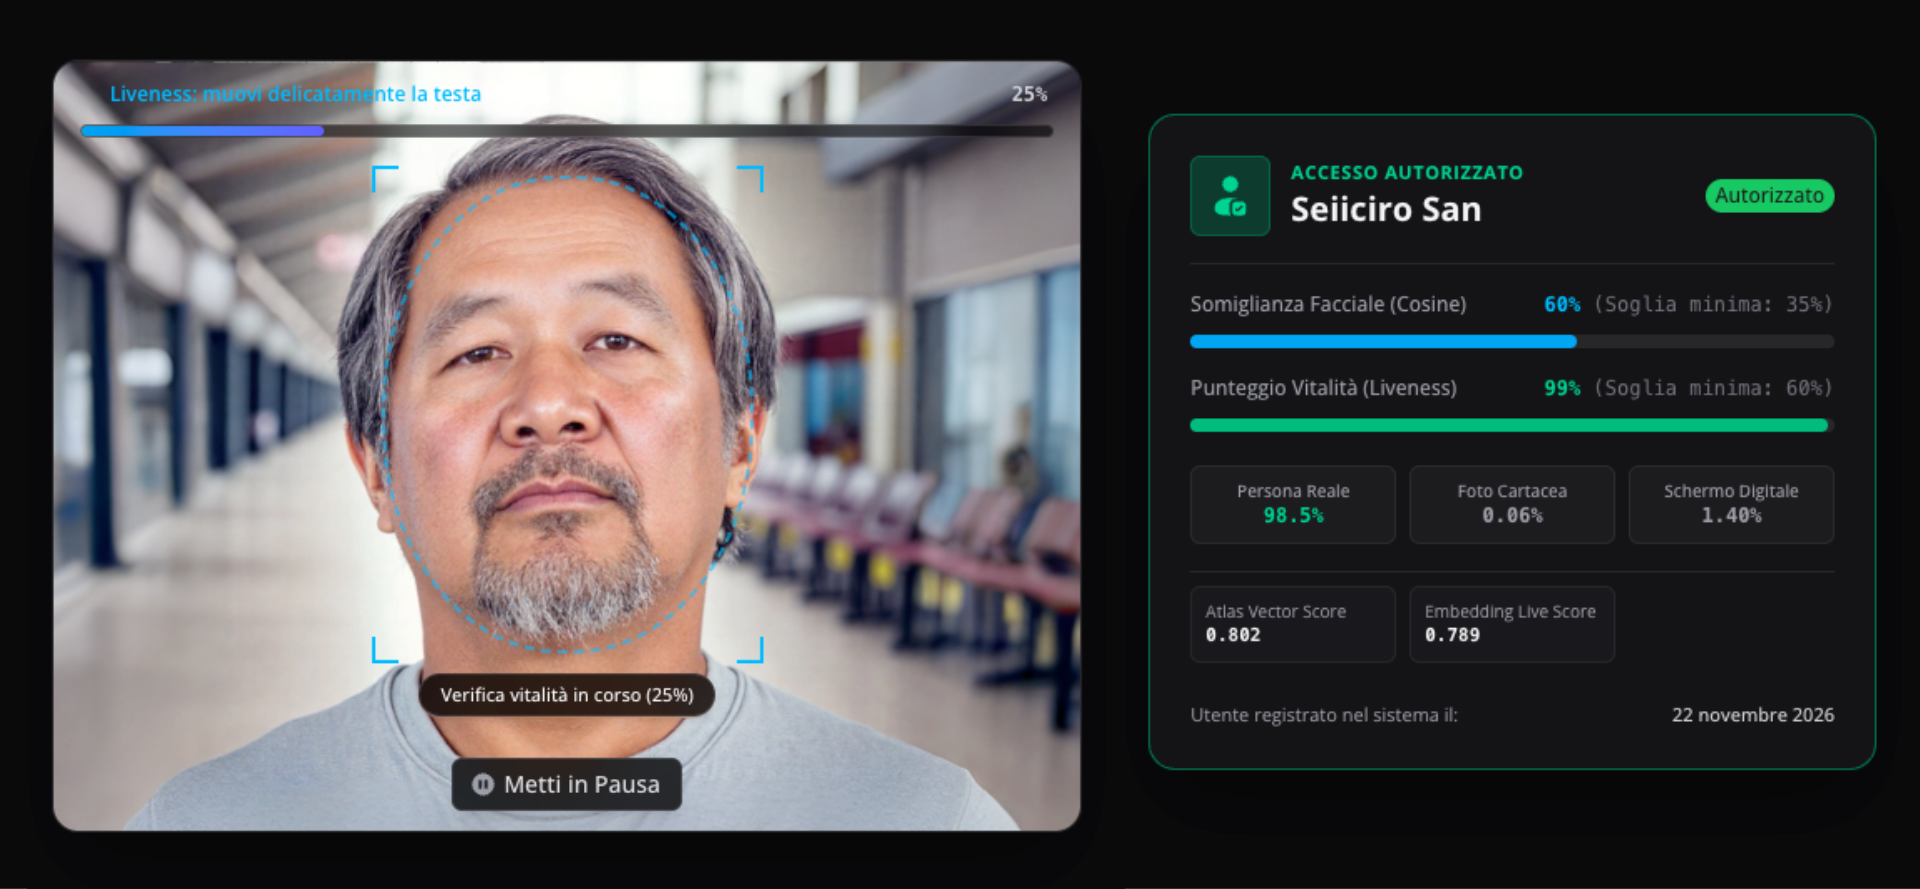
\includegraphics[width=\linewidth]{images/login.png}
    \caption[Interfaccia di \textit{live verification}]{Interfaccia di \textit{live verification}: a sinistra l'acquisizione con la sagoma del volto e l'avanzamento della verifica di vitalità, a destra l'esito della sessione.}
    \label{fig:interfacciaHome}
\end{figure}
La finestra di registrazione utilizza, quando disponibile, la fotocamera posteriore del dispositivo e sovrappone all'anteprima un \textbf{mirino rettangolare} entro cui posizionare la tessera: è questo l'accorgimento citato nel Capitolo~\ref{cap:3.2.1-pipelineCIE}.
In alternativa allo scatto è possibile caricare un file, che viene sottoposto sul client agli stessi controlli di tipo e dimensione applicati dal server (Tabella~\ref{tab:validazioneIngressi}): il controllo lato client serve solo a dare un riscontro immediato all'utente, mentre quello lato server resta l'unico vincolante.
L'esito della registrazione, inclusi gli indicatori di rettifica e contrasto, viene notificato al termine della richiesta.

\begin{figure}[h]
    \centering
    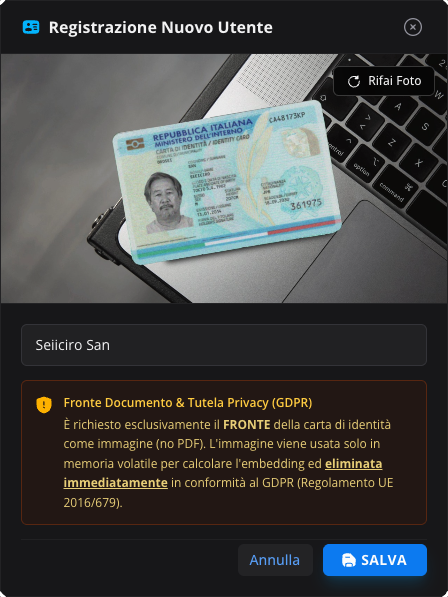
\includegraphics[width=0.6\linewidth]{images/registrazione.png}
    \caption{Finestra di registrazione}
    \label{fig:modaleRegistrazione}
\end{figure}

\paragraph{Acquisizione dei fotogrammi}
L'accesso alla fotocamera avviene tramite il metodo \texttt{getUserMedia()} delle API \textit{MediaDevices}, che richiede il consenso esplicito dell'utente ed è disponibile soltanto in un contesto sicuro, cioè su pagine servite tramite HTTPS o da \texttt{localhost}~\cite{MediaDevicesGetUserMediaMethod2025}.
I vincoli richiesti sono la fotocamera frontale e una risoluzione ideale di $1280 \times 720$ pixel\footnote{Se il dispositivo non è in grado di soddisfarli, la richiesta viene ripetuta senza vincoli, così che la verifica resti possibile anche con fotocamere meno recenti ($RNF3$).}.
Il flusso video è collegato a un elemento \texttt{<video>} visibile, specchiato orizzontalmente soltanto tramite stile grafico per rendere naturale l'inquadratura: i fotogrammi inviati al server non sono specchiati, e corrispondono quindi a ciò che la fotocamera \textbf{acquisisce realmente}.

Ogni fotogramma viene disegnato su un elemento \texttt{<canvas>} nascosto, ridimensionato in modo che il lato maggiore non superi 640 pixel, e codificato in JPEG con qualità $0{,}88$ tramite il metodo \texttt{toBlob()}.
Il ridimensionamento riduce, senza penalizzare il rilevatore, che lavora comunque su un ingresso di $320 \times 320$ pixel (Capitolo~\ref{cap:3.2.2-faceAnalysis}).
Il risultato viene convertito in un \texttt{ArrayBuffer} e inviato come frame binario, secondo la serializzazione asimmetrica definita nel Capitolo~\ref{cap:2.2-architettura}.

\paragraph{Controllo di flusso sul canale WebSocket}
Il metodo \texttt{send()} di un WebSocket non attende che il destinatario abbia elaborato il messaggio: se il client inviasse fotogrammi a ritmo fisso, più velocemente di quanto il server riesca a elaborarli, questi si accumulerebbero nei buffer di rete.
Il server finirebbe così per analizzare immagini sempre più vecchie, e i messaggi di stato mostrati all'utente si riferirebbero a una posa ormai superata.
Per evitarlo, il client adotta un meccanismo di \textit{backpressure} basato su \textbf{un solo fotogramma in transito alla volta} (Listato~\ref{lst:backpressure}).
\begin{lstlisting}[float=htbp, caption={Controllo di flusso con un solo fotogramma in transito (estratto da \texttt{components/CameraScanner.tsx}).}, label={lst:backpressure}]
intervalRef.current = window.setInterval(() => {
  if (isScanCompletedRef.current || ws.readyState !== WebSocket.OPEN) return;
  if (isSendingFrameRef.current) return; // risposta precedente non arrivata

  ctx.drawImage(video, 0, 0, w, h);          // lato massimo 640 px
  isSendingFrameRef.current = true;
  canvas.toBlob(blob => blob?.arrayBuffer()
        .then(buf => ws.send(buf)), "image/jpeg", 0.88);
}, FRAME_INTERVAL_MS);  // 40 ms

ws.onmessage = (event) => {
  isSendingFrameRef.current = false;         // sblocca il frame successivo
  const data: LoginWSMessage = JSON.parse(event.data);
  ...
};
\end{lstlisting}
\\Un \textbf{temporizzatore} propone un nuovo fotogramma ogni $\Delta = 40~\text{ms}$, ma l'acquisizione viene saltata finché il riferimento \texttt{isSendingFrameRef} indica che il server non ha ancora risposto al fotogramma precedente. Il riferimento viene rilasciato all'arrivo di qualsiasi messaggio, compreso un \texttt{ERROR}, oppure se la codifica fallisce.
Poiché il server risponde a ogni fotogramma (Tabella~\ref{tab:messaggiWS}), il ritmo effettivo di invio \textbf{si adatta da solo} alla velocità della rete e del backend, come espresso dall'Equazione~\eqref{eq:frameRateEffettivo}:
\begin{equation}
    \label{eq:frameRateEffettivo}
    f_{\text{eff}} = \frac{1}{\max\left(\Delta, \; T_{\text{rtt}} + T_{\text{frame}}\right)}, \qquad T_{\text{sessione}} \approx \frac{N}{f_{\text{eff}}}
\end{equation}
dove $T_{\text{rtt}}$ è il tempo di andata e ritorno sulla rete e $T_{\text{frame}}$ il tempo di elaborazione di un fotogramma dell'Equazione~\eqref{eq:latenzaFrameOttimizzata}.
Con $\Delta = 40~\text{ms}$ il client non supera i $25~\text{fps}$, e con il buffer di riferimento $N = 35$ la durata minima della verifica è di circa $1{,}4~\text{s}$. Su una rete lenta la sessione si allunga, ma ogni fotogramma analizzato resta attuale.
L'obiettivo è mantenere il ritardo tra il movimento dell'utente e il messaggio corrispondente nell'ordine del centinaio di millisecondi, valore riportato in letteratura come compatibile con l'interazione in tempo reale~\cite{RealtimeBiometricAutthentication}.
La durata effettiva della sessione è oggetto delle misure del Capitolo~\ref{cap:4-risultati}.

\paragraph{Feedback visivo e chiusura della sessione}
Durante la scansione, sopra l'anteprima viene disegnato il componente \texttt{FaceMaskOverlay}: una sagoma ovale tratteggiata che indica dove posizionare il volto, accompagnata da un breve messaggio di stato (Figura~\ref{fig:interfacciaHome}).
Ogni messaggio del server aggiorna l'interfaccia secondo la corrispondenza della Tabella~\ref{tab:feedbackUI}.

\begin{table}[htbp]
    \centering
    \footnotesize
    \renewcommand{\arraystretch}{1.25}
    \begin{tabular*}{\textwidth}{@{\extracolsep{\fill}} >{\raggedright\arraybackslash}p{3.2cm} >{\raggedright\arraybackslash}p{10.0cm} @{}}
        \hline
        \textbf{Messaggio ricevuto} & \textbf{Reazione dell'interfaccia} \\
        \hline
        \texttt{WAITING\_FACE} & Invito a posizionare il volto all'interno della sagoma \\
        \texttt{WAITING\_LIVENESS} & Aggiornamento della barra di avanzamento e della percentuale di verifica \\
        \texttt{ERROR} & Testo dell'errore al posto del messaggio di stato, senza interrompere la scansione \\
        \texttt{SPOOF\_ATTACK}, \texttt{MATCH}, \texttt{NO\_MATCH} & Arresto della scansione, chiusura del canale e visualizzazione dell'esito nella card dei risultati \\
        \hline
    \end{tabular*}
    \caption{Corrispondenza tra i messaggi del server e il riscontro visivo mostrato all'utente.}
    \label{tab:feedbackUI}
\end{table}
La barra di avanzamento utilizza direttamente il campo \texttt{liveness\_progress} calcolato dal server: il client non conosce la dimensione $N$ del buffer, e una diversa configurazione di \texttt{FRAMES\_LIVENESS} si riflette sull'interfaccia senza modifiche al codice.
La card dei risultati mostra anche l'indice di staticità e, per un attacco \texttt{STATIC\_FACE}, la dicitura \emph{Faccia statica}.
Se l'utente \textbf{esce dall'inquadratura} il server azzera il buffer (Capitolo~\ref{cap:3.3-orchestrazione}) e la barra riparte da zero alla ripresa, rendendo esplicito che la verifica richiede una presenza continua davanti alla fotocamera.

Alla ricezione di un esito finale, la funzione \texttt{stopScan} interrompe il temporizzatore, chiude il WebSocket con il codice di chiusura normale \texttt{1000}, ferma le tracce della fotocamera e rilascia l'elemento video: l'indicatore di acquisizione del dispositivo si spegne, segnalando all'utente che le immagini \textbf{non vengono più raccolte}.
La stessa funzione viene eseguita se l'utente mette in pausa la scansione o abbandona la pagina.
Una chiusura anomala del canale, ad esempio con il codice \texttt{1011} inviato dal server in caso di errore interno, viene invece mostrata all'utente con il relativo motivo e la possibilità di ripetere la verifica.
% Cattura frame su Canvas e gestione backpressure WebSocket; Feedback visuale (FaceMaskOverlay, progresso) e networking adattivo
% 5pp